\documentclass[11.5pt]{article}
\usepackage{charter}
\usepackage{fullpage}
\usepackage[colorlinks=false]{hyperref}
\usepackage{ifthen}
\usepackage{comment}
\usepackage[title,titletoc]{appendix}

\bibliographystyle{unsrt}
\usepackage{color}
\usepackage{titlesec}
\usepackage{tikz}
\usepackage{tikzscale}
\usepackage{pgfplots}
\usepackage{nomencl}
\usepackage{amsfonts, booktabs,siunitx}
\usepackage{threeparttable}
\usepackage{tabularx}
\makenomenclature

\usepgflibrary{arrows}
\usetikzlibrary{snakes}
\usetikzlibrary{shapes.geometric}
\usetikzlibrary{patterns}
\usetikzlibrary{shapes,arrows,chains}
\usepgfplotslibrary{patchplots,colormaps}
\usetikzlibrary{calc}
\usetikzlibrary{positioning, fit}
\usetikzlibrary{backgrounds}
\usetikzlibrary{intersections}
\usepackage[]{algorithm2e}

\usepackage{flafter}


\newcommand{\todo}[1]{{\color{blue}#1}}
\newcommand{\cmnt}[1]{{\color{red}#1}}

\newcommand{\sectionbreak}{\clearpage}

% math and cite
\newcolumntype{C}[1]{>{\centering}m{#1}}
\usepackage{rotating}
\newtheorem{thm}{Theorem}
\newtheorem{defn}{Definition}
\newcommand{\refsec}[1]{\S\ref{#1}}
\newcommand{\reffig}[1]{Fig.\ref{#1}}
\usepackage{soul}
\usepackage{amsmath}
\usepackage{url}
\usepackage{amsfonts}
\usepackage{amssymb}
\usepackage{amsthm}
\usepackage{soul}
\usepackage{fullpage}
\usepackage[noend]{algorithmic}
%\usepackage{subfigure}
\usepackage[american]{babel}
%\usepackage{csquotes}
%\usepackage{biblatex}
\usepackage{listings}
\usepackage{caption}
\usepackage{subcaption}


\lstset{emph={long, contract, return, uint256, bool, function, if, true,
    else, using, returns, constant, string, public, namespace, struct, for,
    int,char, typedef, void, double, float, static_cast,
    new},emphstyle=\bfseries\ttfamily, 					basicstyle=\ttfamily,
  moredelim=[is][\color{red}]{^}{^}}

%\lstset{language=C++,
                %basicstyle=\ttfamily\footnotesize,
                %keywordstyle=\color{blue}\ttfamily\footnotesize,
                %stringstyle=\color{red}\ttfamily\footnotesize,
                %commentstyle=\color{green}\ttfamily\footnotesize,
                %morecomment=[l][\color{magenta}]{\#}
%}
%\lstset{%
  %escapeinside={(*}{*)},%
%}

\SetKwProg{Contract}{contract}{ \{}{\}}
\SetKwProg{Function}{function}{ \{}{\}}
\SetKwProg{If}{if}{ \{}{\}}
\SetKwProg{Else}{else}{ \{}{\}}
\newcommand{\String}{\KwSty{string}}
\newcommand{\Public}{\KwSty{public}}
\newcommand{\Returns}{\KwSty{returns}}
\newcommand{\Shared}{\KwSty{shared}}
\newcommand{\Constant}{\KwSty{contant}}
%\addbibresource{reference.bib}

\begin{document}

% ---------------------------------
% Los siguientes comandos son un quickfix para la imposibilidad de compilar este documento usando Babel.
\renewcommand\contentsname{Tabla de contenidos}
\renewcommand\refname{Referencias}
\renewcommand\appendixname{Anexo}
\renewcommand\appendixpagename{Anexos}
\renewcommand{\abstractname}{Resumen}
\renewcommand{\nomname}{Glosario}
\renewcommand{\figurename}{Fig.}
\renewcommand{\tablename}{Tabla}
\renewcommand{\baselinestretch}{1.5}
\newcommand{\dapp}{DApp\xspace}
\newcommand{\pidc}{Protocolo de Incentivos para Desarrolladores\xspace}
% ---------------------------------

\title{
	Libro blanco de Nebulas \\
	\large El sistema operativo con motor de búsqueda en blockchain basado en \textit{rankings}\\
	\small Título original: Nebulas Technical Whitepaper: The value-based blockchain operating system and search engine\\
	\small Traducción: Abril de 2019\\v1.0.0}
\author{Equipo Nebulas}
\date{Abril de 2018\\v1.0.2}

\maketitle

\newpage
\abstract{

Tanto Bitcoin como Ethereum introdujeron satisfactoriamente las ideas de “sistema de dinero electrónico p2p” y “contratos inteligentes” al mundo del blockchain. La industria evoluciona rápidamente, con más aplicaciones emergentes y requerimientos; sin embargo, para las tecnologías blockchain actuales, hemos visto que existen tres desafíos centrales: lograr el establecimiento de una medida de valuación para las aplicaciones en el blockchain, implantar la habilidad de la auto-evolución incorporando los futuros avances en los bloques, y establecer un ecosistema sano a largo plazo, disponible para todos los participantes del mundo blockchain.

  Nebulas apunta a darles curso a estos desafíos. Este libro blanco explica la ideología detrás del diseño técnico y los principios del \textit{framework} de Nebulas; este último incluye:

\begin{itemize}
  \item \textbf{Nebulas Rank (NR)} (\refsec{sec:rank}), un nuevo sistema para la valuación de aplicaciones en el blockchain.
  Nebulas Rank mide la valuación \footnote{N. del T.: \textit{Ranking}, en inglés} de las aplicaciones teniendo en cuenta la liquidez y la propagación tanto de las direcciones como de los contratos inteligentes utilizados en las {\dapp}s de la plataforma Nebulas, en una forma veraz, computable y determinista. Con nuestro nuevo sistema de valuación seremos capaces de ver asomar más {\dapp}s con un uso real en la plataforma Nebulas.


	\item \textbf{Nebulas Force (NF)} (\refsec{sec:nebulasforce}), cuyo fin es el de ofrecer la actualización de los protocolos centrales y de los contratos inteligentes de forma directa en los \textit{main chains}, o cadenas principales. Esto le brindará a Nebulas la capacidad de auto-evolucionar y de incorporar tecnología de punta en sus blockchains, una vez que estén listas para su uso en el mundo real. Con Nebulas Force, los desarrolladores podrán construir aplicaciones sofisticadas en forma rápida, and these applications can dynamically adapt to market changes or community feedback.


	\item \textbf{Developer Incentive Protocol (DIP)} (\refsec{sec:dip}), está pensado para desarrollar nuestro ecosistema blockchain mediante la otorgación de tokens Nebulas, a modo de incentivo, a los mejores desarrolladores de nuestra plataforma, quienes serán determinados mediante nuestro sistema Nebulas Rank. Esto ayudará a recompensar las mejores aplicaciones, y a incentivar a sus desarrolladores a crear más valor, tanto para sí mismos como para Nebulas.


  \item \textbf{Algoritmo de consenso Prueba de Devoción (\textit{Proof of Devotion}, o PoD)} (\refsec{sec:pod}). Para crear un ecosistema sano, Nebulas propone tres puntos clave para su algoritmo de consenso: celeridad, irreversibilidad, y equidad.

  \item \textbf{Motor de búsquedas para {\dapp}s}~(\refsec{sec:search}). Nebulas está construyendo un nuevo tipo de motor de búsqueda para {\dapp}s, basado en el sistema Nebulas Rank. Al usar este motor, los usuarios serán capaces de encontrar las {\dapp}s más útiles y ajustadas a sus necesidades.

\end{itemize}
} %TRADUCIDO
\tableofcontents

\printnomenclature


\nomenclature{NR}{Nebulas Rank}%
\nomenclature{NF}{Nebulas Force}%
\nomenclature{SCS}{Puntaje de Contrato Inteligente}%
\nomenclature{SCR}{Valuación de Contrato Inteligente}%
\nomenclature{PoW}{Prueba de Trabajo}%
\nomenclature{PoS}{Prueba de Participación}%
\nomenclature{PoI}{Prueba de Importancia}%
\nomenclature{PoD}{Prueba de Devoción}%
\nomenclature{DIP}{Protocolo de Incentivo a Desarrolladores}%
\nomenclature{WAA}{Direcciones Semanalmente Activas}%
\nomenclature{BFT}{Tolerante a Faltas Bizantinas}%
\nomenclature{NNS}{Servicio de Nombres de Nebulas}%
\nomenclature{NVM}{Máquina Virtual de Nebulas}

\renewcommand{\nomname}{术语表(按首字母排序)} %TRADUCIDO
\newpage
\section{Introducción}

\subsection{Introducción a la tecnología Blockchain}

La tecnología del blockchain se derivó de la primera moneda digital descentralizada, Bitcoin, que fue conceptualizada por Satoshi Nakamoto en 2008 \cite{Nakamoto2008}. En lugar de ser \textit{acuñado} por una institución bancaria, cada bitcoin se genera a través de algoritmos específicos y computación masiva para asegurar la consistencia de su \textit{sistema de contabilidad}.

Ethereum \cite{buterin2014ethereum} va más allá y proporciona una plataforma informática pública basada en blockchains que incluye un lenguaje Turing-completo. El núcleo de estos sistemas de criptodivisa —representados por Bitcoin y Ethereum— es la tecnología subyacente del blockchain. Con los componentes de cifrado de datos, \textit{timestamping}, consenso distribuido e incentivos económicos, la tecnología de blockchains hace realidad las transacciones entre pares, la coordinación y la colaboración en un sistema distribuido en el que los nodos no necesitan confiar los unos en los otros, resolviendo los problemas comunes a los que se enfrentan las instituciones centralizadas, incluyendo el almacenamiento de datos de alto costo, ineficiente e inseguro.

Cabe señalar que la tecnología de los blockchains no es en sí misma una novedad tecnológica, sino más bien una innovación que combina una serie de tecnologías que incluyen la comunicación entre pares, la criptografía, las estructuras de datos de los blockchains, etc.

\subsection{Desafíos tecnológicos y de negocios}

A medida que más personas se unen en pos del desarrollo de sistemas de autogobierno descentralizados, el mundo observa un aumento dramático del número de proyectos basados en blockchain: más de 2000 proyectos, con activos digitales de carácter global cuyo valor asciende a 90 mil millones de dólares. El número de usuarios de blockchains —propietarios al mismo tiempo de activos digitales— también está aumentando rápidamente: de 2 millones a principios de 2013 a 20 millones a principios de 2017. Para 2020, se espera que el número de usuarios de blockchains y el de propietarios de activos digitales alcance o supere los 200 millones, y para 2025, los 1000 millones.

Con la popularidad de la tecnología blockchain están surgiendo más aplicaciones y casos de uso basados en ellos.  Tales casos se han extendido gradualmente desde las criptodivisas a los contratos inteligentes desarrollados por Ethereum, a la capa de acuerdos globales desarrollada por Ripple, etc. Estos casos también han venido acompañados de crecientes demandas y desafíos sobre los blockchains subyacentes.

\paragraph{Valuación.} Uno de los principales desafíos de los blockchains existentes es la falta de un estándar de valuación. Creemos que ese ecosistema necesita una metodología para valuar tanto a los usuarios como los contratos inteligentes. Las aplicaciones de capas superiores pueden construirse a partir de esta valuación, que les brinda métricas de cada caso particular de uso. En este sentido, en el futuro abundarán las innovaciones en los modelos de negocio que recuerdan el auge de Google en el mundo de Internet.

\paragraph{Actualizaciones en el sistema blockchain.} A diferencia del software tradicional, los sistemas blockchain descentralizados no pueden forzar a sus usuarios a actualizar los clientes o los protocolos. Debido a ello, la actualización de protocolos en los sistemas blockchain a menudo lleva a crear \textit{hard forks} o \textit{soft forks} que resultan en enormes pérdidas para la comunidad, lo que limita más aún los casos de aplicaciones posibles para estos sistemas.

En el caso de Bitcoin, la controversia sobre el problema de escalado de bloques sigue siendo muy grande dentro de la comunidad, lo que dificulta la evolución de su protocolo. La severa insuficiencia de su blockchain ha llevado a una situación única en la que habían casi un millón de transacciones esperando a ser inscritas en los bloques. Los usuarios a menudo tienen que pagar una \textit{tarifa de aceleración de transacciones} exageradamente alta, lo que afecta seriamente su experiencia con el sistema. Por otro lado, aunque el \textit{hard fork} de Ethereum ofrece una solución temporal al problema causado por el DAO, también da lugar a \textit{efectos secundarios} no deseados como los activos duplicados en los blockchain ETH y ETC, y la consecuente división de su comunidad.

\paragraph{La construcción de un ecosistema de aplicaciones en el blockchain.} Con el rápido crecimiento de las aplicaciones distribuidas ({\dapp}s) en el blockchain, la clave para lograr una mejor experiencia de usuario es tener un ecosistema sólido. Es necesario pensar en cómo ayudar a los usuarios a buscar y encontrar la {\dapp} que necesitan a partir de una colección masiva de aplicaciones blockchain, cómo animar a los programadores a desarrollar más {\dapp}s para los usuarios, y cómo ayudarlos en esa tarea. Tomemos como ejemplo Ethereum: cientos de miles de aplicaciones ya han sido construidas sobre Ethereum; sin embargo, una vez que esto aumente el tamaño de las aplicaciones en el App Store, encontrar la {\dapp} apropiada para una tarea dada será un gran desafío.

\subsection{Principios de diseño de Nebulas}

Nos propusimos diseñar un sistema blockchain auto-evolutivo y basado en incentivos para hacer frente a estos retos y oportunidades. Los principios de diseño son los siguientes:

\begin{itemize}
	\item \textbf{Un algoritmo equitativo para definir la medición de la valuación}

Creemos que es necesaria un estándar para la valuación de los datos en la capa inferior de la pila del blockchain, con el fin de ayudar a identificar otras dimensiones de la información, descubriendo así un mayor valor en el mundo blockchain. Presentamos el algoritmo NR (Nebulas Rank) (ver \refsec{sec:rank}) similar al PageRank \cite{Brin2010}\cite{page1999pagerank} de Google), que combina la liquidez, la velocidad, el ancho y la profundidad del capital en los blockchains para proporcionar una valuación equitativa para sus usuarios. NR es la medida de valor en el ecosistema blockchain, en el que los desarrolladores pueden medir la importancia de cada usuario, de cada contrato inteligente y de cada {\dapp} en diferentes escenarios. NR tiene un enorme potencial comercial y puede ser utilizado en búsquedas, recomendaciones, publicidad, y otros campos.

\item \textbf{La auto-evolución del sistema blockchain system y sus aplicaciones}

Creemos que un sistema bien acondicionado, junto a sus aplicaciones, deben ser capaces de auto-evolucionar para poder realizar cómputos más rápidos, tener una mayor resiliencia y una experiencia de usuario mejorada, todo ello con poca intervención humana. Llamamos a esta habilidad auto-evolutiva \textit{Nebulas Force} (ver \refsec{sec:nebulasforce}). En la arquitectura del Sistema de Nebulas, debido a nuestra bien diseñada estructura de bloques, los protocolos centrales pasarán a formar parte de los datos en el blockchain y se actualizarán mediante la adición de datos.

En cuanto a las aplicaciones (contratos inteligentes) en Nebulas, su actualización es posible mediante el acceso de contratos cruzados a las variables de estado almacenadas en la capa inferior de los contratos inteligentes. El blockchain auto-evolutivo de Nebulas proveerá ventajas sobre otros blockchains públicos en términos de potencial de supervivencia y desarrollo; también les permitirá a los programadores brindar respuestas rápidas a cualquier vulnerabilidad mediante estas actualizaciones, lo que ayudará a prevenir las enormes pérdidas económicas vinculadas al \textit{black-hat hacking}.

\item \textbf{La construcción de un ecosistema de aplicaciones blockchain}

Desarrollamos el algoritmo PoD \refsec{sec:pod} basándonos en el concepto de la \textit{devoción de cuentas} en Nebulas. Este algoritmo utiliza NR como medida de valor para identificar aquellas cuentas con gran \textit{devoción} al ecosistema, y les otorga una determinada probabilidad de resultar elegidos como \textit{contables}, en igualdad de condiciones frente a otras cuentas, con el fin de frenar el monopolio en el ejercicio de esa función. También integra en su algoritmo las penalizaciones económicas naturales del consenso PoS para evitar daños maliciosos a llos blockchains públicos, facilitando así, mediante esas dos medidas, la libertad del ecosistema. Las principales características son: mayor velocidad en el consenso y mayor resistencia al fraude que los algoritmos de consenso PoI y PoS.

También estamos desarrollando el algoritmo DIP (\textit{Developer Incentive Protocol}, o Protocolo de Incentivo a Desarrolladores) (véase \refsec{sec:dip}) que aplica a contratos inteligentes y desarrolladores de aplicaciones descentralizadas, y cuyo objetivo es el de premiar a los programadores de contratos inteligentes y {\dapp}s por su gran devoción a la comunidad. Para garantizar la transparencia, un \textit{contador} se encarga de registrar el incentivo en el blockchain.

Basado en Nebulas Rank, se incluye además un motor de búsqueda (véase \refsec{sec:search}) para ayudar a los usuarios a encontrar aplicaciones de calidad en el blockchain.

\end{itemize}

Dado que Ethereum es una exitosa plataforma pública de blockchain, con un ecosistema masivo, Nebulas busca aprender de su excelente diseño, y busca también que sus contratos inteligentes sean totalmente compatibles con el de esa plataforma, para que las aplicaciones nativas allí puedan ejecutarse en Nebulas con un costo de migración cero.

Basándonos en los principios de diseño mencionados, nos esforzamos por construir un sistema operativo de blockchain, y un motor de búsqueda basado en nuestra medición de valor. Este libro blanco describe en detalle las tecnologías embebidas en Nebulas. \refsec{sec:rank} describe Nebulas Rank, un modelo de valuación, y su algoritmo; \refsec{sec:nebulasforce} describe Nebulas Force, un sistema que le brinda la capacidad de auto-evolución de Nebulas; \refsec{sec:dip}, \refsec{sec:pod}, \refsec{sec:search} y \refsec{sec:tools} versan sobre la concepción de Nebulas y el diseño de su ecosistema para aplicaciones blockchain; por último, \refsec{sec:nascoin} plantea una discusión acerca de NAS, la criptodivisa de Nebulas. %TRADUCIDO
\newpage
\section{Nebulas Rank}
\label{sec:rank}

\subsection{Introducción a Nebulas Rank} \label{subsec:value}
Actualmente la tecnología blockchain y su comunidad han crecido hasta llegar a ser un ecosistema a gran escala. Sin embargo, la percepción popular de blockchain en el mundo es todavía algo superficial; no existe aún una forma razonable de evaluar el valor de una entidad (tal como la dirección de un usuario) en el blockchain. Por ende, trabajamos para elaborar una medida universal de valor. Mediante la exploración y el uso de actividades en el blockchain, hemos creado \textbf{Nebulas Rank} un algoritmo a través del cual se puede cuantificar el valor de cada entidad (como la dirección de un usuario). \textbf{Nebulas Rank} está diseñado para:\begin{itemize}
	\item servir como una medida nativa de valor y como un algoritmo central para distintos escenarios fundamentales, como el algoritmo de consenso (véase \refsec{sec:pod}), el Protocolo de Incentivos a Desarrolladores (véase \refsec{sec:dip}) y el motor de búsquedas de blockchain (véase \refsec{sec:search}), entre otros;
	\item inspirar valuaciones diversas y percepciones más profundas en el ecosistema blockchain, de modo de guiar con más precisión las decisionesde negocios y las actividades de investigación.
\end{itemize}
Basándonos en las metas arriba mencionadas, podemos definir la medición de valor de \textbf{Nebulas Rank} desde tres \textit{dimensiones}:
\begin{itemize}

	\item \textbf{Liquidez}, la frecuencia y escala de las transacciones es la primera dimensión que mide \textbf{Nebulas Rank}. Las finanzas son esencialmente actividades que optimizan los recursos sociales a través de la liquidez del capital y que promueven el desarrollo económico. Blockchain establece una red de valor, en el sentido de que a mayor cantidad y escala de transacciones se logra una mayor liquidez, lo que aumenta aún más las transacciones y su escala, formando así un círculo virtuoso.

	\item \textbf{Propagación}, el alcance y la profundidad de la liquidez de los activos es la segunda dimensión que mide \textbf{Nebulas Rank}. En las redes sociales la propiedad de propagación —es decir: la velocidad, el alcance y la profundidad de la transmisión de la información— es un índice clave que muestra la calidad de la red y el crecimiento de los usuarios. El mismo patrón se puede observar en el mundo blockchain: una propagación de gran alcance implica una liquidez de activos más amplia y profunda, lo que mejora la calidad y la escala de los activos.

	\item \textbf{Interoperabilidad} es la tercera dimensión que mide textbf{Nebulas Rank}. Durante la primera etapa de Internet, sólo existían sitios web sencillos y la información estaba aislada. En la actualidad la información se puede enviar desde distintas plataformas y es cada vez más raro encontrar información aislada. Esta tendencia podría entenderse como un proceso de reconocimiento de la información desde una perspectiva dimensional superior. Creemos que el mundo blockchain también sigue un patrón similar, aunque su desarrollo es más rápido. Habrá más información disponible sobre los activos de los usuarios, sobre contratos inteligentes y sobre {\dapp}s. Y, además, todas esas entidades interactuarán con más frecuencia. Por lo tanto, es cada vez más importante que exista una mejor interoperabilidad en el blockchain.

\end{itemize}

Elegimos los registros de transacciones en blockchain como el origen de datos para \textbf{Nebulas Rank} debido a que la \textit{trayectoria} en el mundo de blockchain es más clara y confiable que la del mundo real. Los datos de las transacciones —como las transferencias y las llamadas a contratos inteligentes— quedan registradas en el blockchain. Aun así, no es trivial diseñar algoritmos de valuación para los datos de transacciones en el blockchain, ya que éstas son naturalmente anónimas y poseen una mayor escala de datos que en el mundo real.

A continuación se describen tres propiedades principales para \textbf{Nebulas Rank}:

\begin{itemize}

	\item Veracidad. Una entidad debe pagar un costo razonable para mejorar su valuación, lo que asegura que el algoritmo pueda identificar a los usuarios legítimos y valiosos. Por un lado, en escenarios como el algoritmo de consenso y el DIP, una valuación veraz anima a los usuarios a contribuir de manera honesta con el fin de obtener un \textit{feedback} positivo. Por otro lado, un resultado veraz proporciona una representación jerárquica significativa de todos los usuarios, lo que será útil para los responsables de tomar decisiones;

	\item Computabilidad. Al ser un indicador fundamental, es vital que el resultado de \textbf{Nebulas Rank} sea accesible instantáneamente, lo que requiere una baja complejidad computacional;

	\item Determinismo. Tal como es requerido en escenarios como el algoritmo de consenso y el DIP, el resultado del cálculo de \textbf{Nebulas Rank} debe ser idéntico y replicable en cualquier cliente.

\end{itemize}

A continuación, diseñamos el framework básico de \textbf{Nebulas Rank}. En primer lugar, los registros de transacciones se representan mediante grafos. En el grafo de transacción (grafo de entidades), cada nodo tiene una entidad asignada, y cada arista representa la transferencia entre dos entidades\cite{Tschorsch2015}. El grafo de transacciones encarna el hecho de que la transferencia de dinero entre usuarios conduce al flujo de activos, lo que ayuda a representar los conceptos de liquidez y propagación definidos anteriormente. Mientras tanto, la forma del grafo puede mostrar claramente la interoperabilidad entre los contratos. Mediante el grafo de transacciones derivado, clasificamos los nodos por su centralidad en la red. En el escenario de \textbf{Nebulas Rank}, LeaderRank \cite{Chen2013}\cite{Li2014} es una valuación más razonable que mejora lo ofrecido por PageRank de Google y NCDAwareRank de NEM \cite{nem}.

\subsection{Grafo de transacciones} \label{subsec:txg}
En esta subsección presentamos la forma en que derivamos los grafos de transacciones a partir de su historial.

Primero, para cualquier tiempo $t_0$, tomamos todas las transacciones \textbf{efectivas} entre direcciones individuales durante $[t_0- T, t_0]$ ($T$ es una constante, generalmente establecida en un mes), donde cualquier transacción puede ser representada como una 4-tupla $(s,r,a,t)$, con $s$ como la dirección de origen, $r$ como la dirección de destino, $a$ como el monto de la transferencia y $t$ como el tiempo de bloque. Decimos que una transacción será \textbf{efectiva} si $a>0$ y $s \neq r	$. Así, cualquier transacción \textbf{efectiva} durante $[t_0- T, t_0]$ se puede representar mediante un conjunto de 4-tuplas:

\begin{align}
\Theta(t_0) = \{(s, r, a, t)\ |\ t_0 - T \le t \le t_0\ \land \ a > 0 \land s \neq t \}
\end{align}

Basándonos entonces en $\Theta(t_0)$, construimos a grafo dirigido ponderado simple $G=(V,E, W)$, donde el conjunto de nodos, el conjunto de aristas y la ponderación de cada arista están denotadas por $V$, $E$ y $W$ respectivamente. Cada nodo en $V$ representa una dirección de cuenta individual, y cada arista en $E$ representa la intensidad de transferencias entre las dos direcciones. Las aristas son dirigidas y tienen asignadas las ponderaciones $w_e$ agregando los principales montos $K$ de todas las transacciones relacionadas:

\begin{align}\label{formula:edgeweight}
w_e = \sum_{i=1}^K a_i,\ s.t.\ a_i \in A_e
\end{align}
$A_e$ es un conjunto ordenado que comprende los montos de todas las transacciones desde $s$ hasta $r$ en $\Theta(t_0)$:
\begin{align}
A_e = \{a_i\ |\ e = (s,r) \land (s, r, a_i, t) \in \Theta(t_0) \land (a_i \ge a_j, \forall i \le j) \}
\end{align}

Adicionalmente, sea $N = |V|$, $M = |E|$, donde $|.|$ es el cardinal del conjunto. Para simplificar, cada nodo se representa por un número entero entre $1$ y $N$.

\begin{figure}[h]
\centering
	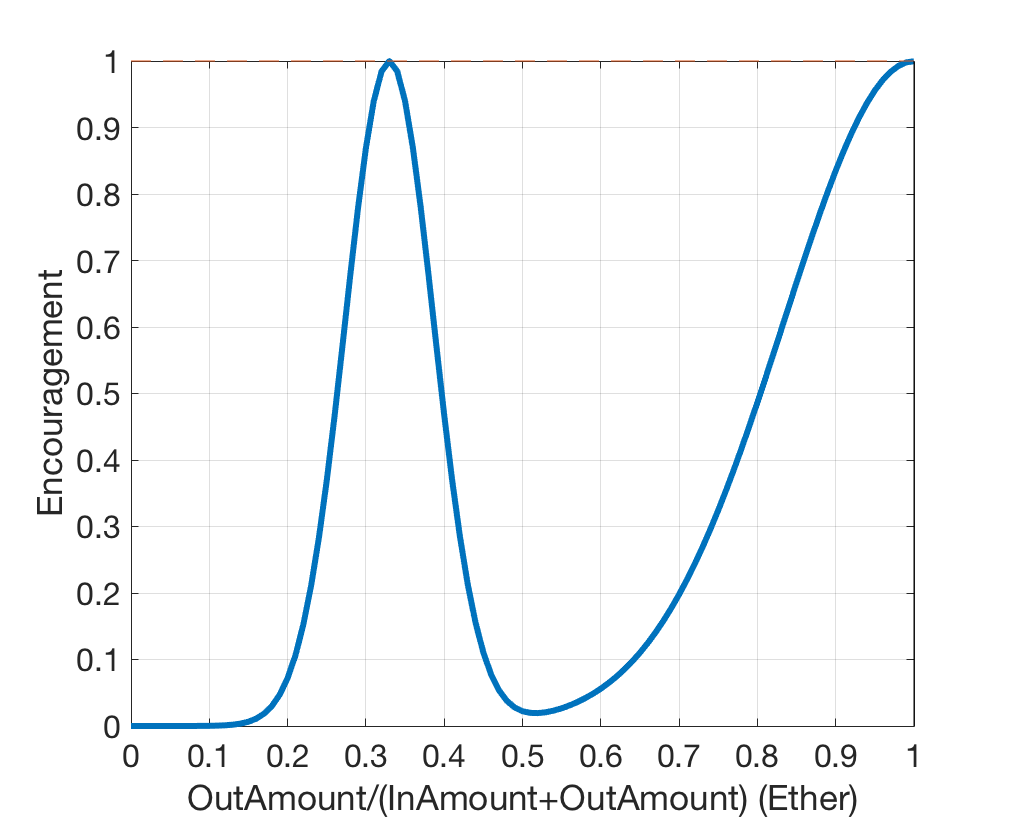
\includegraphics[width=0.55\textwidth]{figs/encouragement_en.png}
	\caption{Función de \textit{estímulo}}\label{fig:encouragement}
\end{figure}

Así, para cada nodo, de acuerdo a sus transferencias entrantes y salientes durante $[t_0\ —\ T,\ t_0]$, se computa la \textit{antigüedad de los depósitos} y se denota esta mediante $C_v$; basándonos en el monto total transferido y haciendo uso de la función \textit{estímulo} que se muestra en la \reffig{fig:encouragement}, se computa el valor \textit{estímulo} y se lo denota mediante $E_v$\footnote{La función estímulo se puede representar como una combinación lineal de dos distribuciones normales, que produce un valor máximo cuando la suma transferida es cero o alguna proporción de las transferencias de ingreso.}; úsense $C_v$ y $E_v$ de los nodos destino para reducir la ponderación de las aristas.

Finalmente, tómese el mayor componente débilmente conectado del grafo y manténganse aquellos nodos que pertenecen a ese componente. Los nodos eliminados reciben, por defecto, el menor puntaje de importancia.

La derivación de grafo descripta arriba contribuye a la propiedad de veracidad definida en \refsec{subsec:value}, cuya evidencia se ofrece en \refsec{subsec:robust}.

Usando el método descripto aquí, el grafo de transacción, donde $T$ representa 30 días y $K=2$, se genera basándonos en los datos transaccionales del blockchain principal de la red Ethereum, desde el bloque \#3629091(aproximadamente del primero de mayo de 2017) hasta el bloque \#3800775(de aproximadamente el 31 de mayo de 2017). Su visualización está disponible en la \reffig{fig:wgc}, y todos los nodos se redimensionan en función de su grado. Se puede observar que algunas casas de cambio famosas suelen interactuar con más cuentas que otras. Además, aún se desconocen las identidades de algunas direcciones que contribuyen con muchas transacciones.

\begin{figure}[htbp]
	\centering
	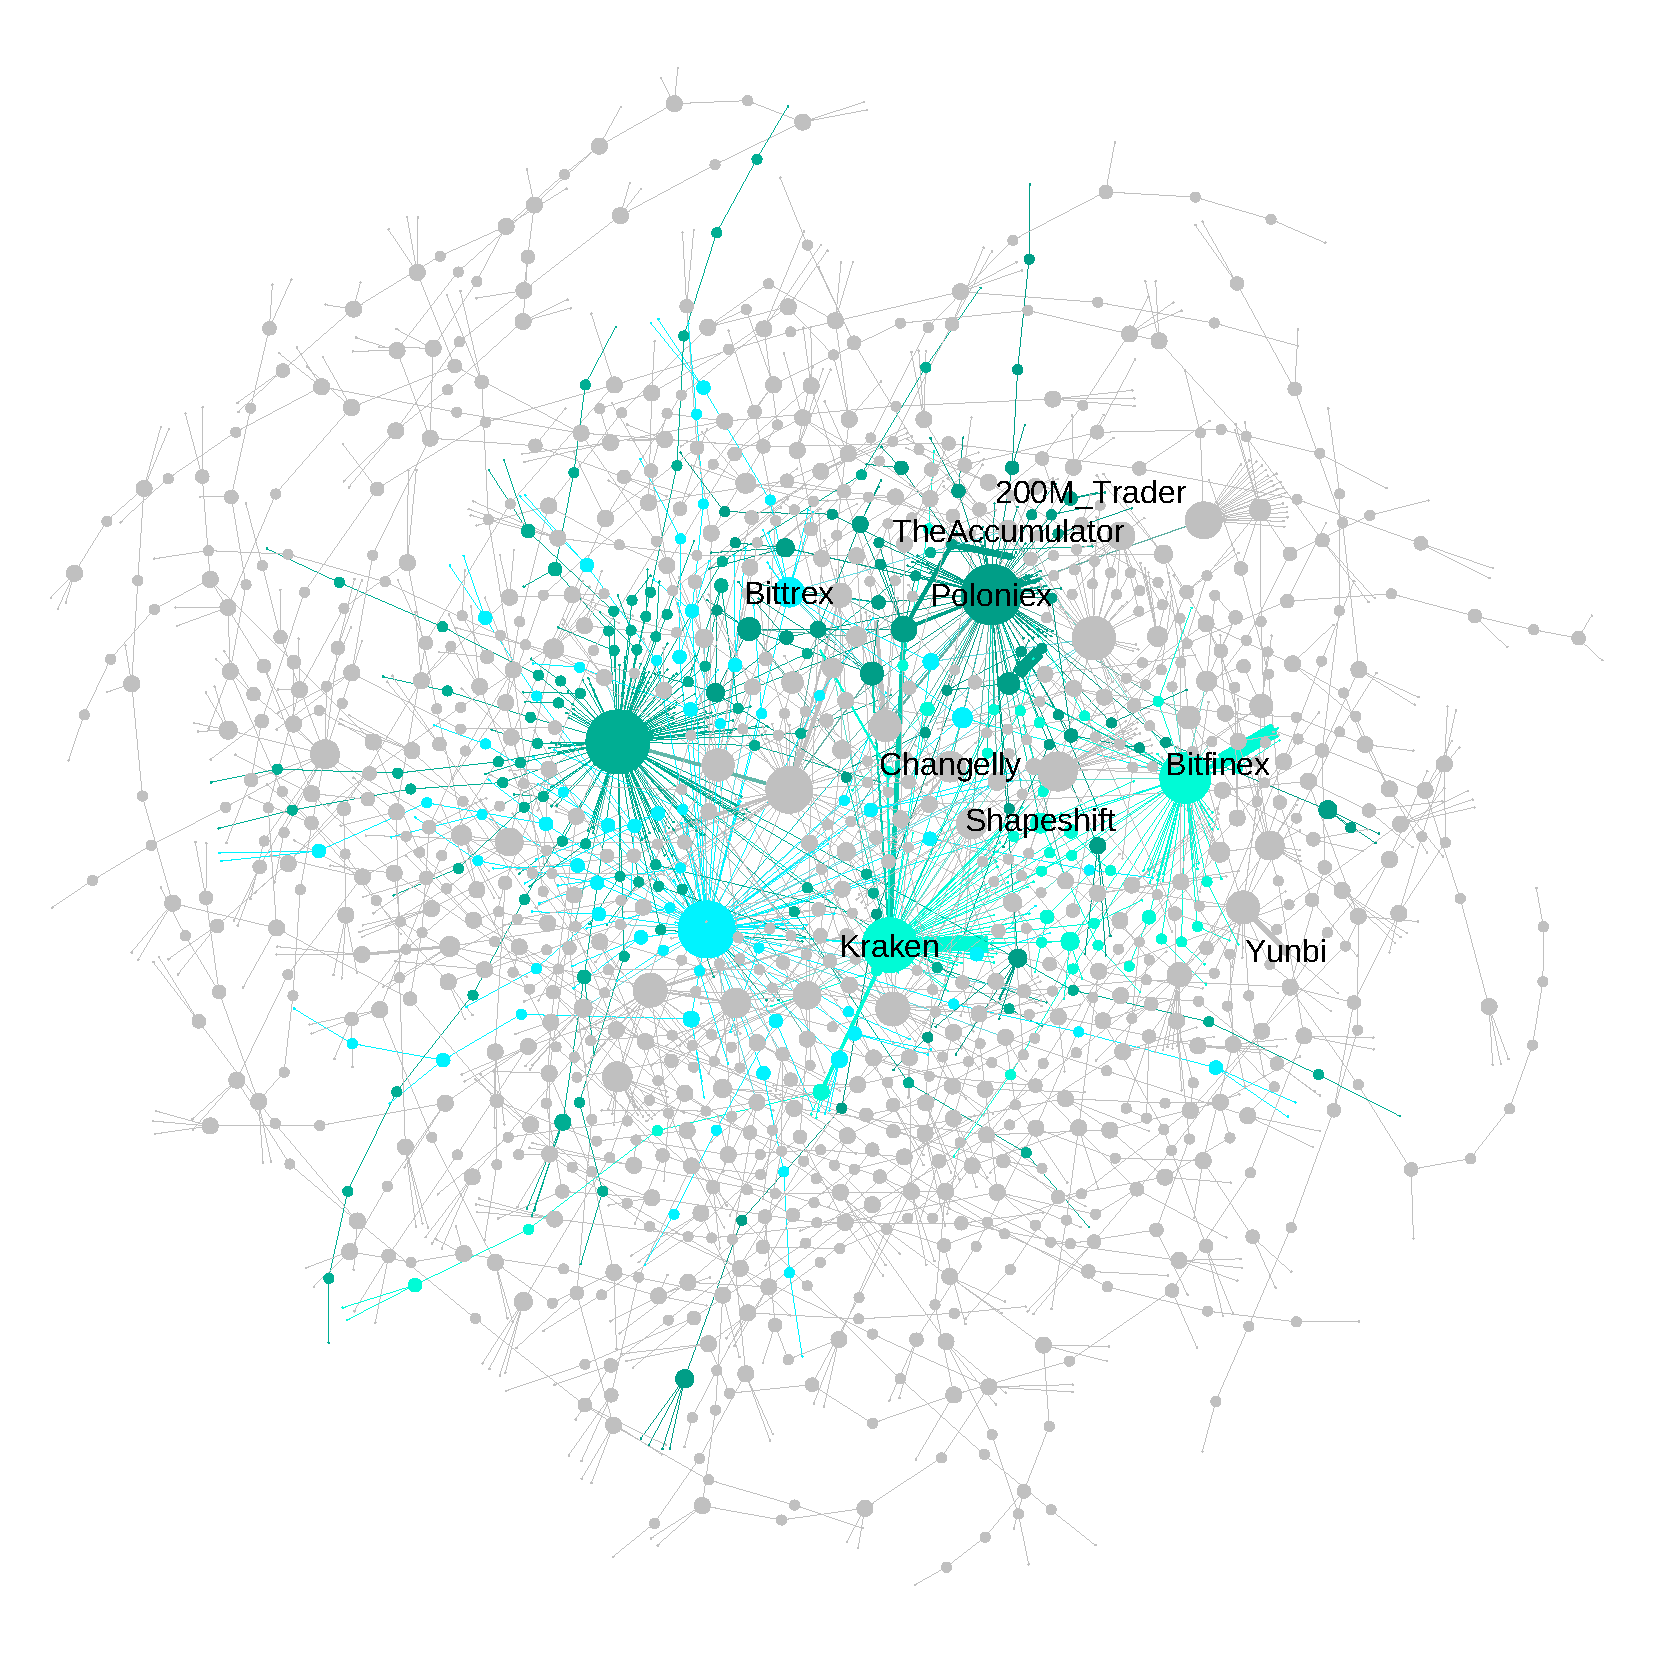
\includegraphics[width=0.85\textwidth]{figs/wgc1.png}
	\caption{Visualización del grafo de transacciones (parcial). \small{La gran escala de transacción (transferencia de capital) en la dirección significa un alto grado de entrada y salida en el nodo, representado por un gran diámetro en la figura. Algunos nodos están etiquetados con nombres, de acuerdo a Etherscan\cite{etherscan}}}\label{fig:wgc}
\end{figure}

\subsection{Algoritmo de valuación} \label{subsec:leaderrank}
Esta subsección explica cómo valuar nodos de acuerdo a su importancia en el grafo transaccional derivado.

Adoptamos LeaderRank\cite{Chen2013}\cite{Li2014} como el principal algoritmo. Primero, añadimos un nodo \textit{ground} con índice $0$ en el grafo de transacciones. Luego establecemos un vínculo bidireccional entre el nodo \textit{ground} $0$ y el resto de los nodos $i$ ($1 \leq i \leq N$), ponderando mediante la siguiente fórmula:
\begin{align}\label{formula:weight1}
w_{i,0} = \alpha( max\{ \sum_{w_{j,i} \neq 0} w_{j,i} - \sum_{w_{i,j} \neq 0} w_{i,j} , 0\} + \lambda C ), \forall i \in [1,N]
\end{align}
\begin{align}\label{formula:weight2}
w_{0,i}	= \beta ( \sum_{w_{i,m} \neq 0} w_{i,m} + \mu C), \forall i \in [1,N]
\end{align}
$C$ es la mediana del conjunto $\{w_{i,j} | w_{i,j} \neq 0, 0\leq i,j \leq N\}$, y $\alpha, \beta, \mu, \lambda$ son parámetros.

El esquema de ponderación puede explicarse de esta forma: los nodos con mayor cantidad de transferencias de ingresos obtienen aristas con mayor ponderación dirigidas desde el nodo \textit{ground}; los nodos con mayores transferencias absolutas (saldo resultante de restar los egresos a los ingresos) generan aristas con mayor ponderación, dirigidas al nodo \textit{ground}.

El esquema de ponderación puede explicarse de la siguiente manera: los nodos con más ingresos reciben aristas con más ponderación desde el nodo \textit{ground}; los nodos con mayores ingresos absolutos (ingresos menos egresos), generan aristas con mayor ponderación dirigidas al nodo \textit{ground}.

El proceso de cómputo de LeaderRank es similar al de PageRank, lo que puede ser entendido como el cálculo del estado de convergencia de un proceso de Markov. La única diferencia es que, luego de añadir el nodo \textit{ground}, ya no es necesario considerar el factor de amortiguación de PageRank\cite{Brin2010}\cite{page1999pagerank}. Esto es, luego de construir la matriz $H$ de acuerdo a la fórmula (\ref{formula:matrix}), el proceso de cómputo se itera hasta lograr convergencia, como se ve en la fórmula (\ref{formula:iteration}), con ajustes iniciales definidos por la fórmula (\ref{formula:init}). Finalmente, el puntaje de valuación del nodo \textit{ground} se distribuye uniformemente a todos los demás nodos, lo que produce la puntuación final para cada uno de ellos.
\begin{align} \label{formula:iteration}
	P^{t+1} = H \times P^{t}; P^1=[0, \frac{1}{N}, \frac{1}{N}, \dots, \frac{1}{N}]^T
\end{align}
\begin{align} \label{formula:matrix}
	h_{ij} = \frac{w_{(j,i)}}{\sum_k w_{(j,k)}}
\end{align}
\begin{align} \label{formula:init}
\forall v \in V, P^*_v \leftarrow P^*_v + \frac{P^*_{\mathcal{G}}}{N}
\end{align}

Suponemos que LeaderRank puede satisfacer la valuación y la propiedad algorítmica definida en \refsec{subsec:value}.
\begin{itemize}
	\item El resultado de LeaderRank puede ser entendido como el flujo en cada nodo dentro del equilibrio dinámico de una red de intercambio de dinero, lo que coincide con la valuación de \textbf{Nebulas Rank}: \textit{liquidez}, \textit{propagación} e \textit{interoperabilidad};
	\item El esquema de ponderación definido por las fórmulas (\ref{formula:weight2}) y (\ref{formula:weight1}) hace que sea más difícil de atacar (véase la discusión en \refsec{subsec:robust}), lo que satisface la propiedad de \textit{veracidad};
	\item LeaderRank puede ser calculado por iteración de potencia. Dado que la red es muy dispersa, la complejidad de la computación matricial no debería ser alta, lo que satisface las propiedades \textit{computable} y \textit{determinista}.
\end{itemize}


\subsection{Resistencia a la manipulación}\label{subsec:robust}
Veracidad, o resistencia a la manipulación, es la meta más desafiante y significativa de \textbf{Nebulas Rank}. Veamos algunos de los métodos posibles de manipulación:
\begin{enumerate}
	\item Bucle de transferencias: el atacante realiza transferencias sobre una topología de bucle, lo que permite que el mismo dinero circule sobre las mismas aristas repetidamente. Así, el atacante espera elevar la ponderación de las aristas asociadas;
	\item Transferencias a direcciones aleatorias, lo que espera lograr que el grado de egresos del nodo Sybil se incremente, y con ello la propagación de fondos;
	\item Formar un componente independiente de red con direcciones controladas por el atacante. Así, éste pretende ser un nodo central;
	\item Interactuar frecuentemente con direcciones de casas de cambio importantes, es decir, transferir el mismo dinero desde y hacia una o más direcciones de casas de cambio importantes, de modo de lograr una mejor posición estructural en la red.
\end{enumerate}

\textbf{Nebulas Rank} mitiga la manipulación a través de los siguientes mecanismos:
\begin{itemize}
	\item Gracias a las \textit{ventanas} móviles de $T$ bloques, el atacante no puede incrementar su valuación en el corto plazo;
	\item Dado que la ponderación de las aristas se decide por medio de las transacciones asociadas de mayor monto, transferir dinero a lo largo de una topología en bucle no incrementa ilimitadamente la ponderación de las aristas. Entretanto, de acuerdo al muestreo de datos en \refsec{subsec:txg}, $91\%$ de aristas corresponden a menos de dos transacciones, respectivamente. Así $K=2$ es una elección razonable para mantener la intensidad de la información de las aristas mientras se resiste la transferencia en bucle;
	\item Para lograr una mayor \textit{antigüedad en los depósitos}, el usuario necesita mantener el dinero en su dirección durante un cierto lapso de tiempo, lo que reduce la velocidad de este ataque;
	\item Con el fin de obtener el máximo valor de \textit{antigüedad de los depósitos}, tal como se ve en la \reffig{fig:encouragement}, la cuenta necesita enviar más de lo que ingresó o bien transferir sólo un pequeño porcentaje de sus ingresos; así, al intentar falsificar el flujo de dinero, el atacante verá reducirse rápidamente sus depósitos;
	\item A raíz de que sólo se seleccionan los componentes más grandes, otros componentes independientes —incluyendo el falsificado— quedarán filtrados. Según los datos de la muestra en \refsec{subsec:txg}, existen $453,285$ nodos y $970,577$ aristas, con $1,169$ componentes. En el componente más significativo, hay $449,746$ nodos, que representan $99.2\%$ del número total. En el segundo componente más significativo, hay sólo $133$ nodos, que representan $0.03\%$. Así, al seleccionar el componente más significativo, se mantiene gran parte de la actividad normal de la red mientras se filtran los componentes menores y las falsificaciones;
	\item Comparado a los algoritmos de valuación de sitios web tales como PageRank y NCDawareRank\cite{Nikolakopoulos2013}, el mecanismo definido por las \ref{formula:weight2} y \ref{formula:weight1} es más conservador en los nodos con pocos ingresos; esto es, los nodos con pocos ingresos obtienen enlaces más débiles con el nodo \textit{ground}. En el grafo de transacciones de blockchain es más probable que se generen nodos con bajos ingresos, y con sólo realizar transferencias a nodos aleatorios no basta para incrementar su grado de ingresos. De modo que \textbf{Nebulas Rank} puede incrementar la dificultad en realizar manipulaciones.
\end{itemize}

Luego, las siguientes conclusiones se basan en el grafo de transacciones de Ethereum en mayo de 2017.

Primero, algunas direcciones de \textbf{Nebulas Rank} se listan en la tabla \ref{table:nr}\footnote{Fuente del dominio: Etherscan\cite{etherscan}}. Puede observarse que las direcciones de las casas de cambio y algunas otras cuentas con un alto rendimiento de transacciones se valúan como nodos principales.

%\newpage
\begin{table}[!htbp]
\centering
\caption{\textbf{Las 10 direcciones principales} de \textbf{Nebulas Rank}, entre otras}
\label{table:nr}
\begin{tabular}{llllll}\toprule
\begin{tabular}[c]{@{}l@{}}Valuación\\ (Orden)\end{tabular} & Dirección                                                                                    & Nebulas Rank & Dominio          & Egreso (Ether) & Ingreso (Ether) \\
1  & \begin{tabular}[c]{@{}l@{}}0x267be1c1d684f78cb4f\\ 6a176c4911b741e4ffdc0\end{tabular} & 0.449275     & Kraken\_4   & 3214232.06  & 350008.00   \\
2  & \begin{tabular}[c]{@{}l@{}}0xd4c5867cec094721aab\\ c3c4d0fd2f2ac7878c79a\end{tabular} & 0.093798     &             & 58000.00    & 100947.00   \\
3  & \begin{tabular}[c]{@{}l@{}}0x027beefcbad782faf69f\\ ad12dee97ed894c68549\end{tabular} & 0.049277     & QuadrigaCX  & 207440.11   & 65606.40    \\
4  & \begin{tabular}[c]{@{}l@{}}0x0ee4e2d09aec35bdf08\\ 083b649033ac0a41aa75e\end{tabular} & 0.046831     &             & 56465.00    & 60087.96    \\
5  & \begin{tabular}[c]{@{}l@{}}0xc257274276a4e539741\\ ca11b590b9447b26a8051\end{tabular} & 0.037628     &             & 1071105.93  & 1434106.72  \\
6  & \begin{tabular}[c]{@{}l@{}}0xa53e0ca7d246a764993\\ f010d1fde4ad01189f4e6\end{tabular} & 0.033488     &             & 7764.68     & 3201.00     \\
7  & \begin{tabular}[c]{@{}l@{}}0xf259e51f791e9ed26e8\\ 9b6cae4a7c6296bfbd0b8\end{tabular} & 0.033481     &             & 3307.00     & 7731.30     \\
8  & \begin{tabular}[c]{@{}l@{}}0xf195cac8452bcbc836a\\ 4d32cfb22235af4ac1e9c\end{tabular} & 0.026343     &             & 10863.87    & 2315.69     \\
9  & \begin{tabular}[c]{@{}l@{}}0x94435d12c51e19d5b5c\\ 8656763f9069d37791a1a\end{tabular} & 0.024970     &             & 12938.58    & 15858.90    \\
10 & \begin{tabular}[c]{@{}l@{}}0x7580ba923c01783115d\\ 79975d6a41b3d38eff8d5\end{tabular} & 0.021670     &             & 263000.00   & 364793.49   \\
16 & \begin{tabular}[c]{@{}l@{}}0xcafb10ee663f465f9d10\\ 588ac44ed20ed608c11e\end{tabular} & 0.004995     & Bitfinex\_1 & 360000.00   & 1435858.40  \\
51 & \begin{tabular}[c]{@{}l@{}}0xd94c9ff168dc6aebf9b\\ 6cc86deff54f3fb0afc33\end{tabular} & 0.000868     & yunbi\_1    & 1179224.74  & 1202539.53  \\
64 & \begin{tabular}[c]{@{}l@{}}0x70faa28a6b8d6829a4b\\ 1e649d26ec9a2a39ba413\end{tabular} & 0.000590     & Shapeshift  & 52501.81    & 651933.49   \\
\bottomrule
\end{tabular}
\end{table}
\newpage

Luego, observamos la relación entre el monto de la transacción y \textbf{Nebulas Rank}. Dado que la transferencia en blockchains puede entenderse como un \textit{flujo de intercambio de dinero en la red} (según el trabajo de \cite{Borgatti2005}), el grado de los nodos, es decir, la suma de las ponderaciones de las aristas adyacentes, es una métrica de centralidad adecuada para dicho flujo de red. Desde la perspectiva de cada nodo, el grado, es decir, el monto absoluto de las transacciones (ingresos menos egresos), representa la información local dentro de un salto y refleja el flujo de dinero histórico sobre las direcciones correspondientes. Así, esto podría tomarse como base para los algoritmos de valuación. La relación entre el monto de la transacción y \textbf{Nebulas Rank} se muestra en la \reffig{fig:nrio}: ningún nodo puede adquirir una valuación alta con un monto de transacción bajo; los nodos con un monto de transacción alto aún necesitan cumplir con otras condiciones para obtener una valuación alta, lo que confirma a grandes rasgos la propiedad de veracidad de \textbf{Nebulas Rank}.

\begin{figure}[!htbp]
	\centering
	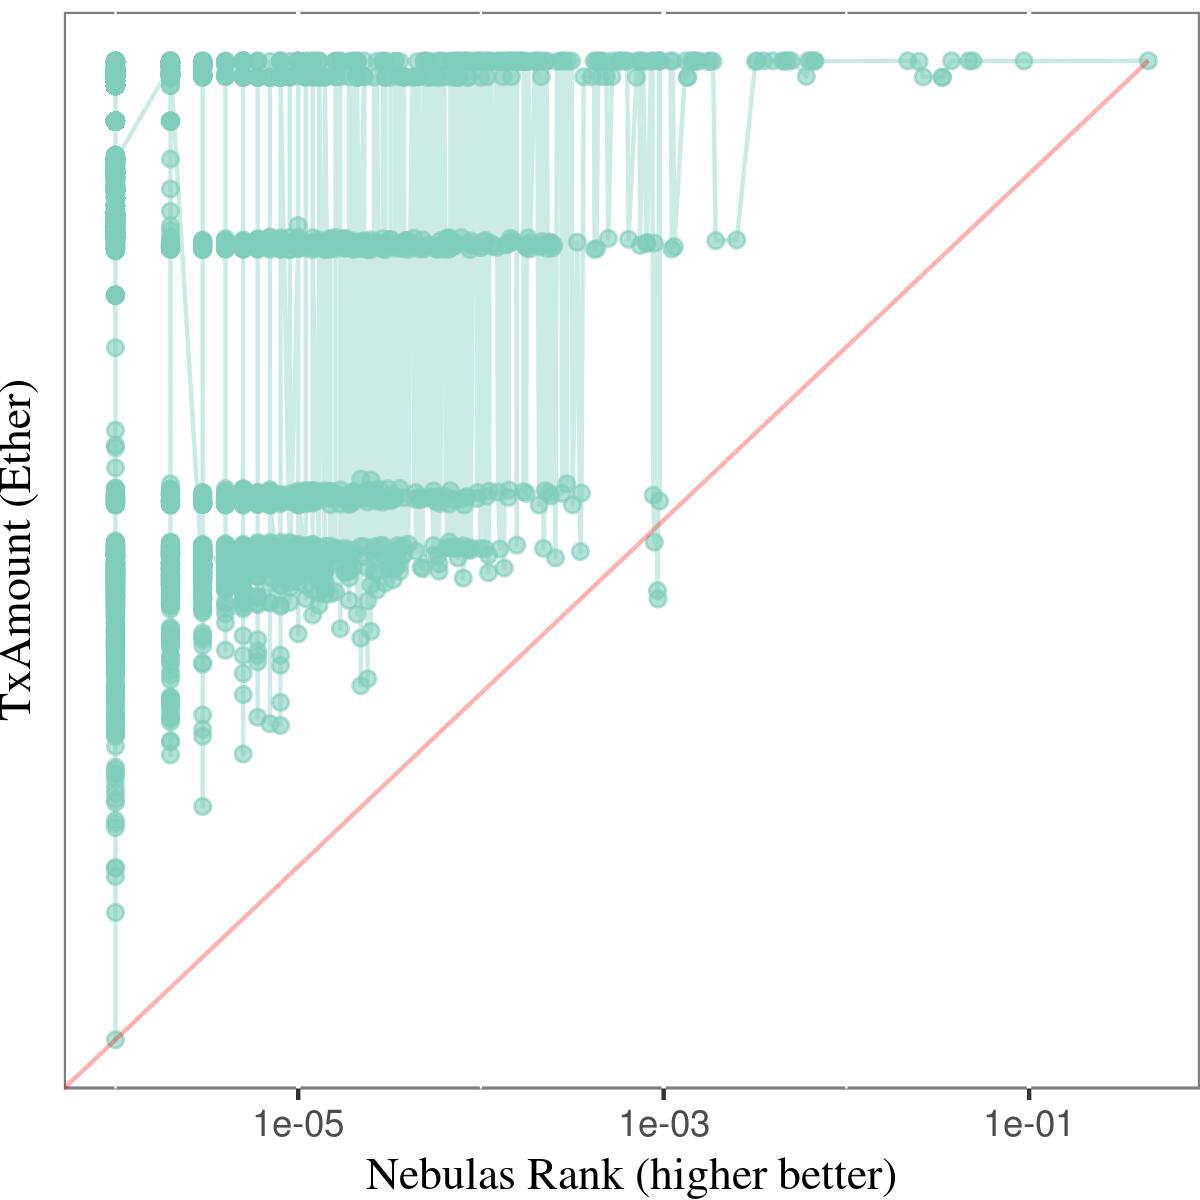
\includegraphics[width=0.50\textwidth]{figs/MAY_lr.png}
	\caption{Nebulas Rank versus monto de transacción \small{El eje de abscisas representa la valuación (\textit{rank value}), y el eje de ordenadas representa el monto de las transacciones; ambos ejes se presentan en escala logarítmica. La línea diagonal muestra que el monto de la transacción y la valuación son directamente proporcionales. Un buen algoritmo debe hacer que los puntos caigan lo menos posible en la parte inferior derecha de la diagonal, para evitar la existencia de nodos con transacciones de montos bajos y con alta valuación.}}\label{fig:nrio}
\end{figure}

De acuerdo con el simple análisis anterior, se puede deducir que los tres primeros tipos de manipulación pueden ser filtrados eficazmente por métodos específicos. Por lo tanto, finalmente, sólo necesitamos simular el último tipo y observar si se produce un efecto de resistencia. El atacante elige un nodo ligado a una casa de cambio de renombre para crear transferencias en bucle durante $X$ veces. Cada bucle de transferencia se compone de dos fases: primero el atacante transfiere $Y$ ETH a la casa de cambio a través de una nueva cuenta provisoria; luego el atacante recupera su dinero a través de otra dirección. La topología y el proceso atacantes se demuestran en la \reffig{fig:loop}. Este tipo de ataque explota el hecho de que el servicio de una casa de cambio está dispuesto a establecer vínculos con cualquier nodo a un costo muy bajo. Si bien es cierto que los nodos normales pueden realizar transferencias regulares con las casas de cambio, ninguno de estos casos mejoran la liquidez monetaria efectiva, y deben ser distinguidos de las operaciones normales.
\begin{figure}[!ht]
	\centering
	%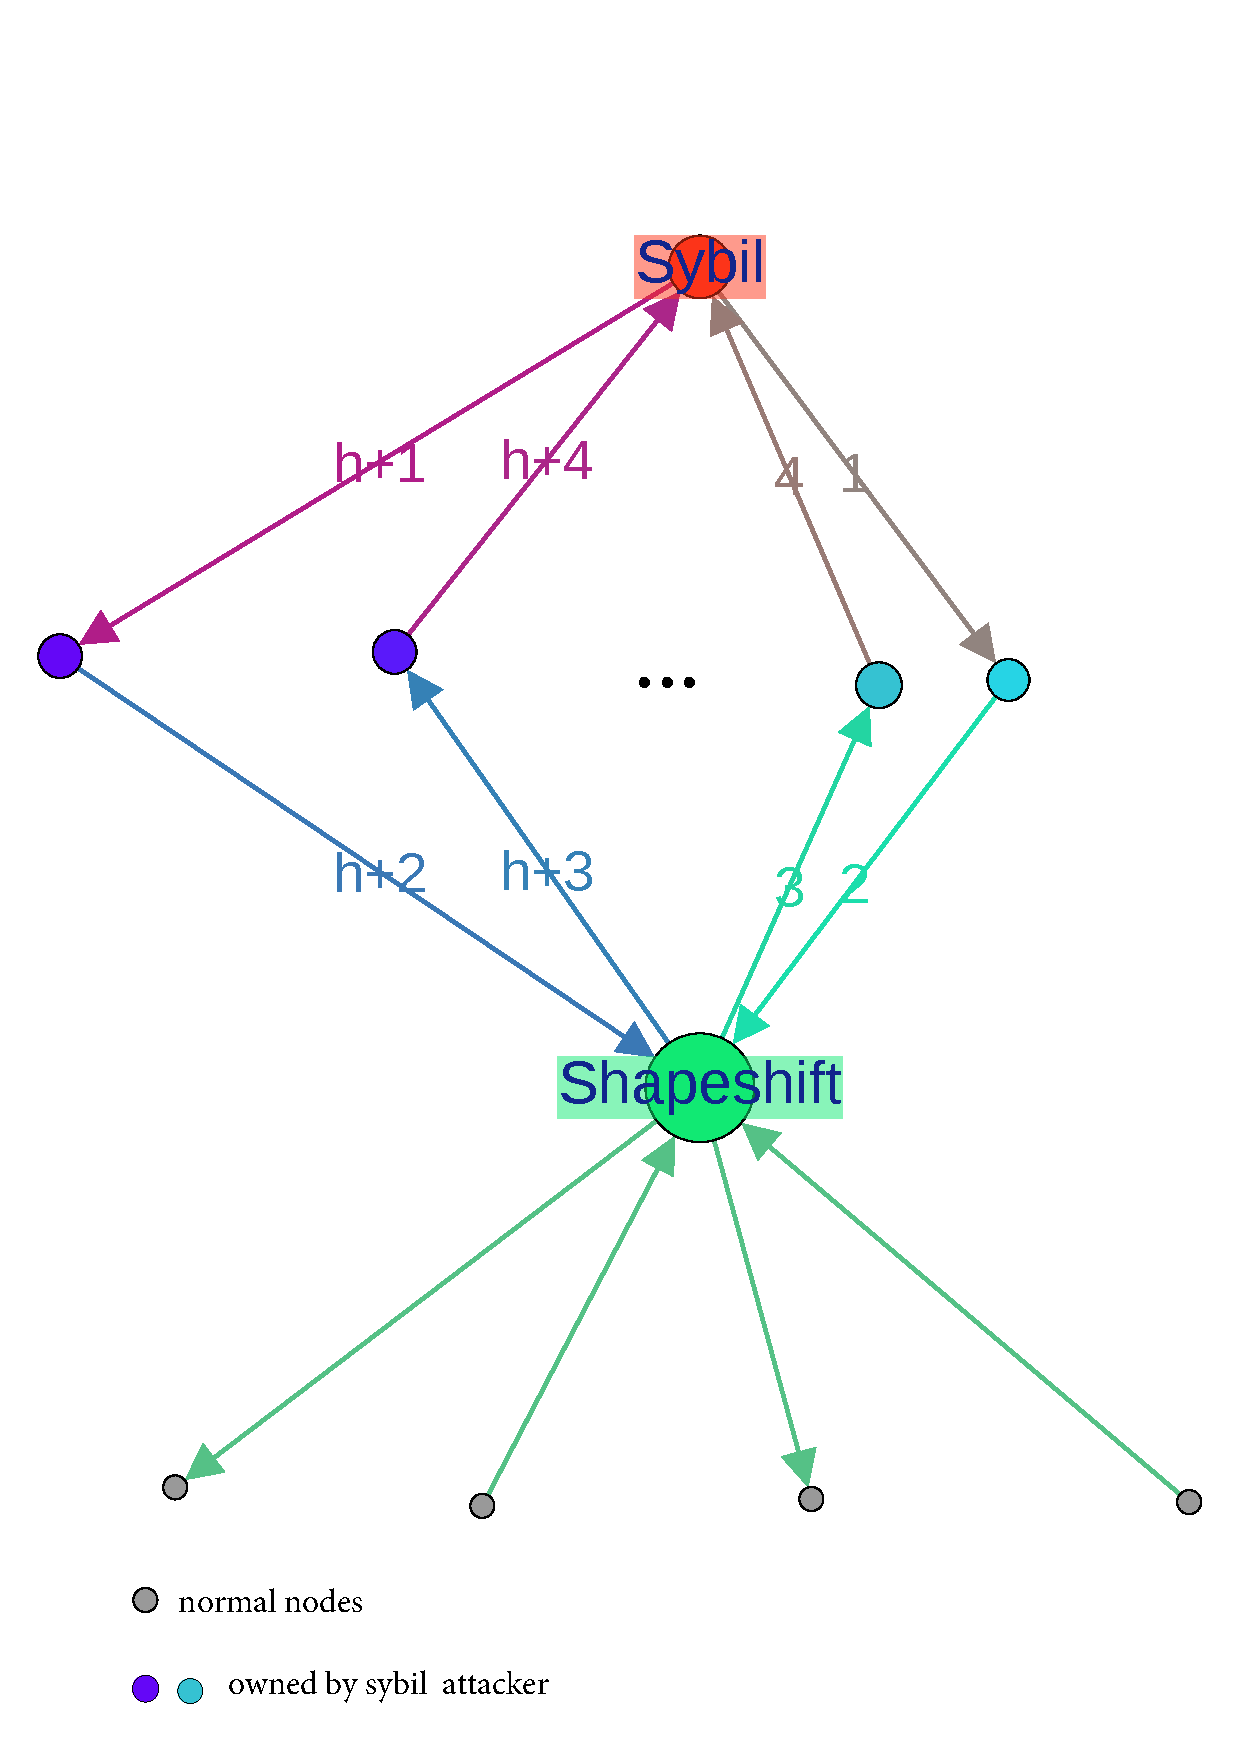
\includegraphics[width=0.35\textwidth]{figs/attack.pdf}
  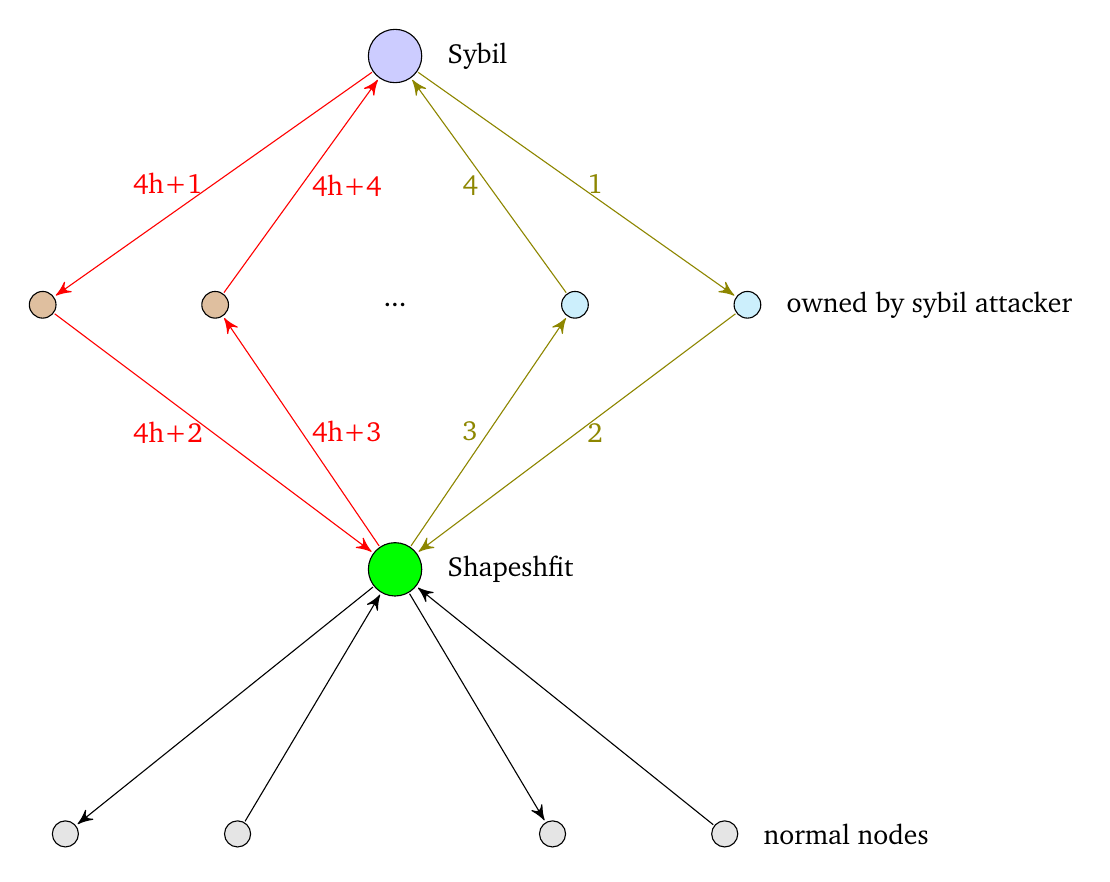
\begin{tikzpicture}
  \pgfmathsetmacro{\YMD}{3}
  \pgfmathsetmacro{\XMD}{2}
\tikzset{
  hnode/.style={draw, circle, on grid, align=center, minimum height=2ex},
  base/.style={draw, circle, on grid, align=center, minimum height=4ex},
  sybil/.style={draw, circle, on grid, align=center, minimum height=4ex, fill=blue!20},
  normal/.style={draw, circle, on grid, align=center, minimum height=1ex, fill=gray!20},
  coord/.style={coordinate, on grid, node distance=6mm and 25mm},
}
%
\tikzset{>=stealth',
  every join/.style={->}, very thick}

       \node [base, fill=green!=20] (ss) at (0, 0) {} node[right
       = 1ex of ss] {Shapeshfit};

       \node (dot) at ($(ss.north) + (0, \YMD)$) {...};

       \node [sybil] (sy) at ($(dot.north) + (0, \YMD)$) {} node[right=1ex of
       sy]{Sybil};

       \node [hnode, fill=brown!50] (hh4) at($(dot.west) + (-\XMD, 0)$){};
       \node [hnode, fill=brown!50] (hh1) at ($(hh4.west) + (-\XMD, 0)$){};

       \node [hnode, fill=cyan!20] (h4) at ($(dot.east) + (\XMD, 0)$){};
       \node [hnode, fill=cyan!20] (h1) at ($(h4.east) + (\XMD, 0)$){} node
       [right = 1ex of h1]{owned by sybil attacker};

       \node [coord] (c) at($(ss.south) + (0, -\YMD)$) {};

       \node [normal] (n2) at ($(c.west) + (-\XMD, 0)$){};
       \node [normal] (n1) at ($(n2.west) + (-\XMD, 0)$){};
       \node [normal] (n3) at ($(c.east) + (\XMD, 0)$){};
       \node [normal] (n4) at ($(n3.east) + (\XMD, 0)$){} node [right=1ex of
       n4] {normal nodes};

       \draw[->, color=red] (sy) -- (hh1) node [midway, left]{4h+1};
       \draw[->, color=red] (hh4) -- (sy) node [midway, right]{4h+4};
       \draw[->, color=olive] (h4) -- (sy) node [midway, left]{4};
       \draw[->, color=olive] (sy) -- (h1) node [midway, right]{1};

       \draw[->, color=red] (hh1) -- (ss) node [midway, left]{4h+2};
       \draw[->, color=red] (ss) -- (hh4) node [midway, right]{4h+3};
       \draw[->, color=olive] (ss) -- (h4) node [midway, left] {3};
       \draw[->, color=olive] (h1) -- (ss) node [midway, right]{2};

       \draw[->] (ss) -- (n1);
       \draw[->] (n2) -- (ss);
       \draw[->] (ss) -- (n3);
       \draw[->] (n4) -- (ss);

\end{tikzpicture}

	\caption{Esquema de un ataque de bucle utilizando una dirección de casa de cambio \small{En la figura vemos el primer y el $h$-ésimo ataques de bucle. El nodo seleccionado pertenece a la casa de cambio Shapeshift; las etiquetas de las aristas indican la secuencia temporal; el monto transferido entre los nodos controlados por un atacante Sybil y el de Shapeshift es $Y$ ETH; Hay $X$ transferencias de bucle durante la manipulación.}}\label{fig:loop}
\end{figure}

Elegimos la dirección 0x70faa28a6b8d6829a4b1e649d26ec9a2a39ba413 que pertenece a la casa de cambio Shapeshift. Los resultados se muestran en la  \reffig{fig:antiManipulation}: 1) como se ve en la \reffig{subfig:deposit}, ningún algoritmo es capaz de prevenir que mejore la valuación del atacante cuando éste invierte más capital, mientras el grafo de transacciones definido en \refsec{subsec:txg} reduce los efectos del ataque. \textbf{Nebulas Rank} no sólo puede escoger nodos con un alto rendimiento de transacciones, sino que además resiste esta manipulación hasta cierto límite; 2) tal como se muestra en la \reffig{subfig:times}, con el atacante creando más transferencias en bucle, el grafo de transacciones definido en \refsec{subsec:txg} puede hacer que la valuación del atacante empeore; la razón para ello es que ese grafo toma en consideración factores como la \textit{antigüedad de los depósitos} y el valor \textit{estímulo}. Entretanto, \textbf{Nebulas Rank} podría fortalecer estos factores, generando así más resistencia contra la manipulación.

\begin{figure}[htbp]
	\centering
	\begin{subfigure}{\linewidth}
		\centering
		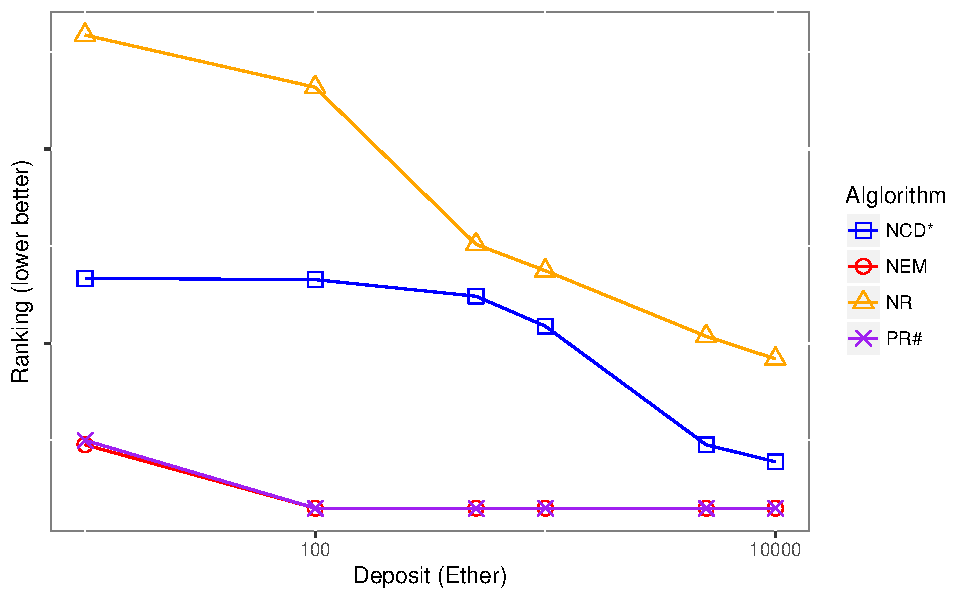
\includegraphics[width=0.7\textwidth]{figs/AttackDeposit.pdf}
		\caption{El efecto del tamaño del capital del atacante en su valuación, con el número de transferencias en bucle fijado en $5,000$. \small{(Los ejes están en escala logarítmica)}}
		\label{subfig:deposit}
	\end{subfigure}

	\begin{subfigure}{\linewidth}
	    \centering
		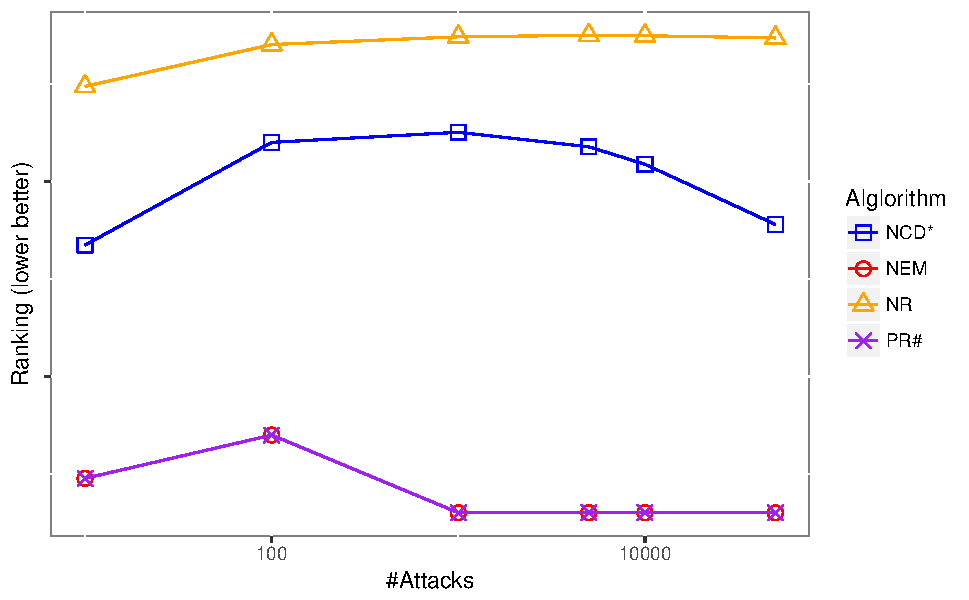
\includegraphics[width=0.7\textwidth]{figs/AttackTimes.pdf}
		\caption{El efecto del número de transferencias en bucle en la valuación del atacante, con su capital fijado en $\Xi5000$ \small{(Los ejes están en escala logarítmica)}}\label{subfig:times}
	\end{subfigure}

	\caption{Resistance contra la manipulación} \label{fig:antiManipulation}
	\caption*{\footnotesize{El método de ataque se muestra en la \reffig{fig:loop}; el eje de abscisas representa el capital del atacante, y el eje de ordenadas, el orden de su valuación (un orden de valuación mayor significa que el atacante falla en obtener mayor valuación, indicando una mayor resistencia por parte del algoritmo)  \\
	NR: el grafo de transacciones se define en \refsec{subsec:txg}, y el algoritmo de valuación se describe en \refsec{subsec:leaderrank}; \\
	%PR$^*$: The transaction graph is defined at \refsec{subsec:txg}, PageRank algorithm;\\
	NCD$^*$: el grafo de transacciones se define en \refsec{subsec:txg}, junto al algoritmo NCDawareRank; \\
	NEM: el grafo de transacciones es presentado por \cite{nem}, junto a NCDawareRank\\
	PR$^{\#}$: el grafo de transacciones es presentado por \cite{nem}, junto al algoritmo PageRank\\
	El factor de atenuación de PageRank es de 0,15; El algoritmo de clustering utilizado por NCDawareRank es pscan\cite{chang2017mathsf}, $\eta=0.75$, $\mu=0.1$}}
\end{figure}

\subsection{Trabajos relacionados} \label{subsec:related}

La centralidad, el índice de valuación base, es el concepto más estudiado en la ciencia de redes desde hace décadas\cite{newman2010networks}. Hay un cuerpo de literaturas que introducen varias centralidades, incluyendo la centralidad de los grados\cite{freeman1979set}, la centralidad de los valores propios\cite{bonacich1972factoring}, la centralidad de Katz\cite{katz1953new}, la centralidad de cercanía\cite{sabidussi1966centrality}, la centralidad intermedia\cite{freeman1977set}\cite{freeman1978centrality}\cite{freeman1991centrality}\cite{noh2004random}\cite{newman2005measure}, PageRank\cite{Brin2010}, HITS\cite{kleinberg1999authoritative}, SALSA\cite{Science2001}, etc.

Además, hay algunos trabajos fundamentales que tratan de clasificar y revisar claramente estas medidas mediante un marco de trabajo unificado\cite{Borgatti2005}\cite{Borgatti2006}\cite{Lu2016}. Al diseñar \textbf{Nebulas Rank}, antes de adoptar centralidad, primero es necesario considerar la propiedad del grafo. El escenario del grafo de transacciones de blockchain es mayormente similar a la red de flujos monetarios mencionada en \cite{Borgatti2005}. Sin embargo, los algoritmos relacionados mencionados por su trabajo —tales como flujo de centralidad intermedia\cite{freeman1991centrality} y paseo aleatorio de centralidad intermedia (también conocido por \textit{current betweenness centrality})\cite{newman2005measure}— son intensivos en computación y no satisfacen la propiedad \textit{computable} en la gran escala del grafo de transacciones de Blockchain.

Desde el lanzamiento de Bitcoin\cite{Nakamoto2008} en 2009, los investigadores han realizado algunos análisis estadísticos y empíricos sobre el grafo de transacciones de Bitcoin\cite{Ron}\cite{Haslhofer}\cite{NielKondor2014}\cite{Baumann2014}, y algunos de ellos utilizan la estructura del grafo de transacciones para discutir el anonimato de esa red\cite{Meiklejohn2013}\cite{Ober2013}\cite{pham2016anomaly}\cite{Fleder2015}\cite{Ferrin2015}. Después del lanzamiento y popularización de otras criptodivisas, se llevó a cabo un análisis del grafo de transacciones sobre más blockchains\cite{Chang2017}\cite{Anderson2016}. \textbf{Nebulas Rank} adopta sus conceptos de grafos de transacciones; esto es, Grafo de Entidades en \cite{Tschorsch2015}, con algunas revisiones menores. Es decir, cada cuenta, o conjunto de cuentas que pertenecen a la misma gente, se mapea como un nodo, y cada arista dirigida representa la intensidad de la transferencia entre dos cuentas. En realidad, antes de que se inventara un sistema blockchain como Bitcoin, los científicos intentaron estudiar algunas redes financieras entre bancos y entidades de comercio mundial.\cite{propper2008towards}\cite{Boss2004}\cite{Serrano2007}\cite{Bech2008}\cite{Fagiolo2009}\cite{Morten2006}\cite{Boss2004a}\cite{Krempel2002}\cite{Serrano2003}. Comparando con el grafo de transacción en blockchain, estas redes financieras estudiadas tempranamente se definen no sólo por la transferencia de actividades, sino también por información adicional (como préstamos). Además, la escala de esas redes es mucho menor. Para concluir, rara vez se han realizado trabajos de investigación que propongan un método de valuación personalizado para un grafo de transacción a gran escala, especialmente un grafo de transacciones en el blockchain.

El trabajo más relevante con \textbf{Nebulas Rank} es el esquema de Prueba de Importancia NEM\cite{nem}. Éste adopta NCDawareRank\cite{Nikolakopoulos2013}, que explota el efecto de clustering de la topología de red, como el algoritmo de valuación, con su algoritmo de clustering basado en el de SCAN\cite{xu2007scan}\cite{shiokawa2015scan}\cite{chang2017mathsf}. Aunque la estructura de comunidad existe en el grafo de transacción y debería ser útil para manejar los nodos de spam, no se garantiza que todos los nodos en el mundo Blockchain, controlados por una entidad en el mundo real, estén mapeados en un solo cluster, lo que deja mucho espacio para la manipulación. Además, \cite{Fleder2015} utiliza PageRank\cite{Brin2010}\cite{page1999pagerank} como métrica auxiliar para el descubrimiento de direcciones interesantes, y para el análisis de sus actividades. No obstante ello, su trabajo no brinda un marco de trabajo automatizado para la identificación de nodos importantes. En vez de ello, éste depende del análisis subjetivo, lo que no concuerda con el contexto de \textbf{Nebulas Rank}.

El algoritmo que elegimos es LeaderRank\cite{Chen2013}\cite{Li2014}. Es una variante simple pero efectiva de PageRank\cite{Brin2010}\cite{page1999pagerank}; en ésta, cada nodo tiene asignado un parámetro de teleportación idéntido, mientras LeaderRank agrega un llamado \textit{nodo ground}, asignándole distintos parámetros de teleportación por cada nodo. El esquema de ponderación de \textbf{Nebulas Rank} está tomado parcialmente del diseño de \cite{Li2014}, lo que permite que los nodos con mayor grado de ingresos tengan más chances de teleportación. Adoptar el algoritmo LeaderRank podría arrojar resultados más afines al escenario de Blockchain. %TRADUCIDO
\newpage
\section{Nebulas Force}
\label{sec:nebulasforce}

Nebulas Force (NF) se utiliza para describir la capacidad evolutiva tanto del sistema blockchain como de sus aplicaciones. Como primera fuerza motriz del sistema blockchain y del desarrollo de sus aplicaciones, Nebulas Force incluye tres aspectos que son: la Máquina Virtual Nebulas (\textit{Nebulas Virtual Machine}, NVM), la actualización del código del protocolo en el sistema blockchain, y la actualización de los contratos inteligentes que corren en dicho sistema.

En Nebulas, introduciremos LLVM para implementar la Máquina Virtual de Nebulas (NVM). El código de protocolo y el código de los contratos inteligentes se compilarán en \textit{NVM bytecode}, que se compila y optimiza dinámicamente con la función de compilación JIT (just-in-time) de LLVM y que, finalmente, se ejecutarán en un entorno \textit{sandbox}. Mientras tanto, con la arquitectura modular de LLVM, los desarrolladores pueden utilizar sus lenguajes de programación favoritos para implementar contratos inteligentes más seguros y de mayor rendimiento, proporcionando a los usuarios, así, diversas aplicaciones descentralizadas.

Para el proceso de actualización del código de protocolo, Nebulas colocará éste dentro de la estructura de los bloques, añadiendo a ellos los datos adicionales necesarios, de modo de evitar cualquier \textit{fork}.

La capacidad de actualización de NF y los protocolos básicos quedará gradualmente abierta a la comunidad de Nebulas a medida que esta crezca y pueda definir por sí misma el camino evolutivo de Nebulas y los objetivos de las actualizaciones.

Con la ayuda de su tecnología central, y con la apertura de NF a la comunidad, Nebulas será un espacio en permanente evolución, y con un potencial de desarrollo prácticamente infinito. Por ejemplo, será posible actualizar una serie de parámetros incluyendo los del algoritmo NR, el total de incentivos PoD, el algoritmo de consenso y la tasa de producción de nuevos \textit{tokens} sin necesidad de actualizar el código de los clientes.

Los contratos inteligentes se consideran usualmente como fijos, sin soporte a actualizaciones. Con la ayuda del diseño de almacenamiento subyacente de los contratos inteligentes en Nebulas, que permiten la consulta de variables de estado entre contratos, es posible crear actualizaciones para ellos. Esta solución es además muy amigable con los desarrolladores, permitiéndoles así brindar una respuesta rápida a cualquier vulnerabilidad o error, lo que en definitiva ayuda a prevenir pérdidas cuantiosas de dinero causadas por errores o \textit{hackers}. %TRADUCIDO
\subsection{Máquina Virtual de Nebulas (\textit{Nebulas Virtual Machine}, NVM)}
\label{sec:nvm}

LLVM \cite{llvm} es el componente central de la NVM, y el bytecode LLVM se utiliza como bytecode NVM.

El bytecode de la NVM se compila de forma dinámica, se optimiza por medio del JIT LLVM y se ejecuta en el entorno \textit{sandbox} de NVM. Gracias a esta arquitectura, la performance y la seguridad del código del núcleo y de los contratos inteligentes en Nebulas se puede mejorar continuamente mediante LLVM.

LLVM es una colección de \textit{toolchains} y tecnologías de compilación altamente modulares, que se utilizó previamente como \textit{framework} de compilación de código en Google, Apple y muchas otras empresas. LLVM proporciona representaciones intermedias neutrales (LLVM IR) y una infraestructura de compilación acorde, y ofrece un nuevo conjunto de estrategias de compilación con respecto a esta infraestructura, incluyendo la optimización de LLVM IR, la generación de código de LLVM IR a bytecode LLVM y la ejecución directa del bytecode LLVM en diferentes plataformas de hardware a través del JIT LLVM, tal como se muestra en la \reffig{fig:llvm}. \\

\begin{figure}[h]
\centering
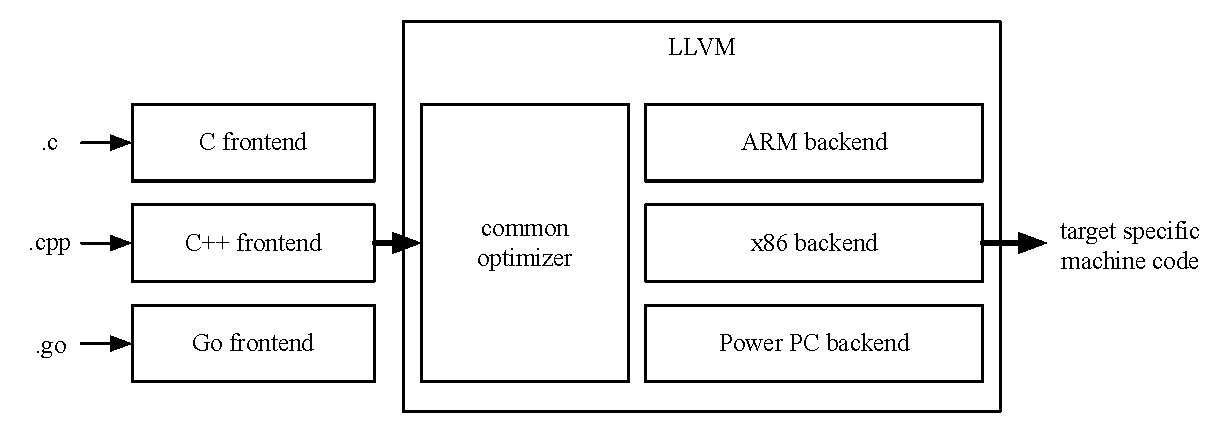
\includegraphics[width=10cm]{./figs/llvm}
\caption{LLVM}
\label{fig:llvm}
\end{figure}

Desarrollamos la NVM basándonos en LLVM (véase \reffig{fig:nvm}). En primer lugar, proporcionamos las librerías API subyacentes para blockchain. Luego, creamos un \textit{frontend} para el compilador, disponible en diferentes lenguajes tales como Solidity, JavaScript, C, C++, Go, etc. A continuación, utilizamos el \textit{toolchain} proporcionado por LLVM para generar el bytecode LLVM. Finalmente, este bytecode LLVM se ejecuta en un \textit{sandbox} proporcionado por NVM a través del motor JIT de LLVM.

\begin{figure}[h]
\centering
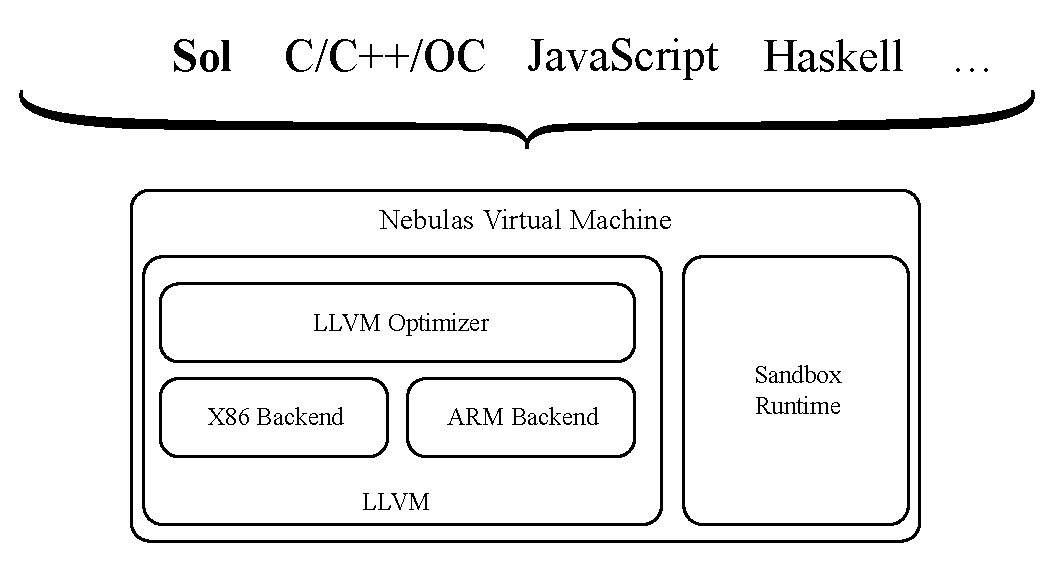
\includegraphics[width=10cm]{./figs/nvm}
\caption{Máquina Virtual de Nebulas}
\label{fig:nvm}
\end{figure}

La Máquina Virtual de Nebulas es la piedra angular de Nebulas Force. Cuando se libera un nuevo código de protocolo o un contrato inteligente, el bytecode LLVM se genera luego de que el nuevo código es compilado por LLVM en NVM, y es liberado al blockchain. Una vez confirmado allí, el nuevo código será compilado y optimizado por LLVM JIT, y colocado en el sandbox para reemplazar el código viejo y ser ejecutado, tal como se muestra en la \reffig{fig:nvm-process}.

\begin{figure}[h]
\centering
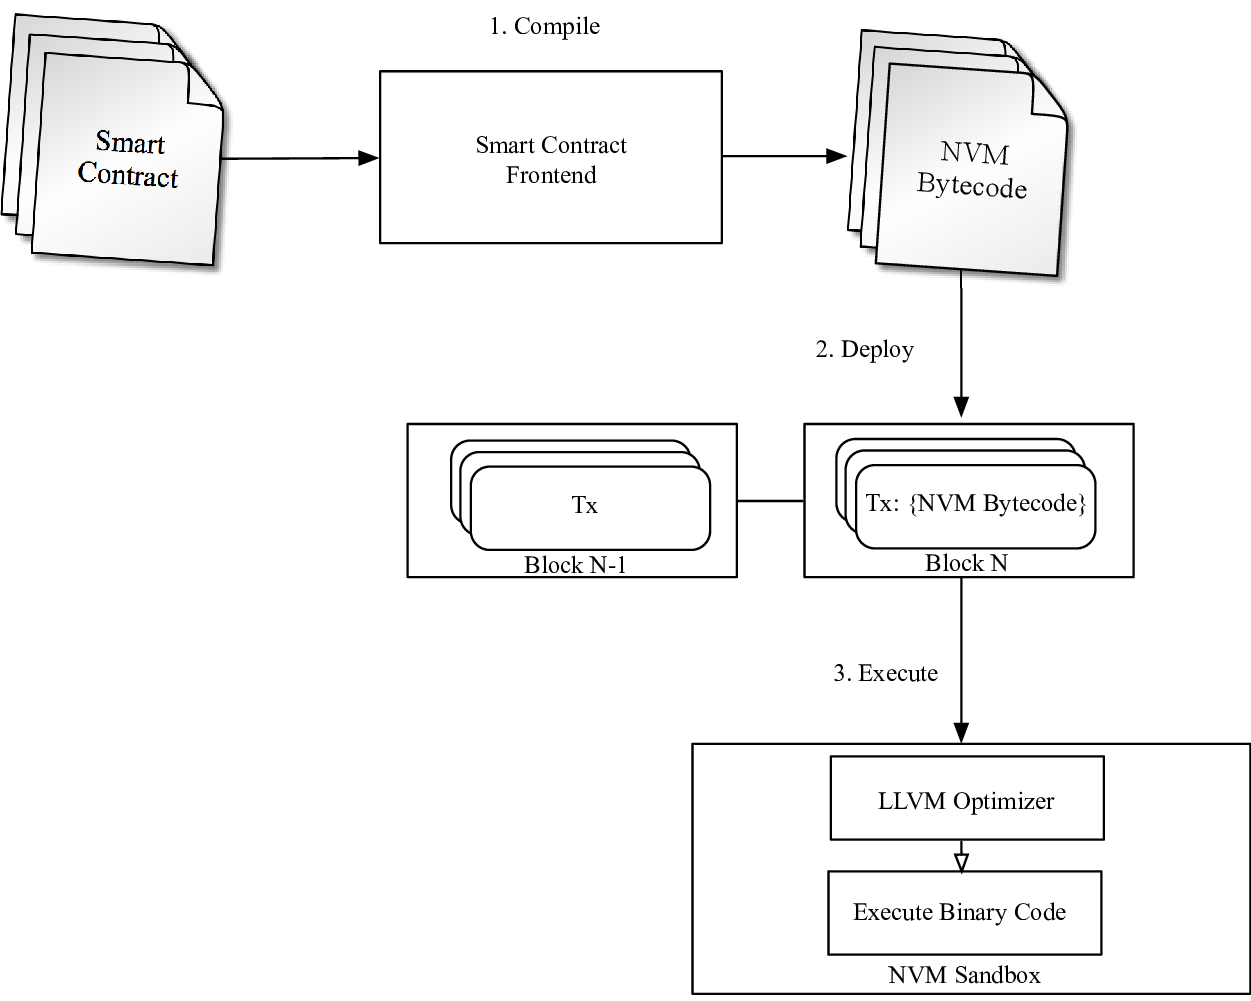
\includegraphics[width=10cm]{./figs/nvm-process}
\caption{El mecanismo de operación de la Máquina Virtual de Nebulas}
\label{fig:nvm-process}
\end{figure}

Con LLVM (véase \reffig{fig:llvm}), NVM también ayuda a los desarrolladores a escribir contratos y aplicaciones inteligentes por medio de sus lenguajes de programación favoritos, como Solidity, JavaScript, e incluso Haskell. Además de estos populares lenguajes, NVM también da soporte a lenguajes personalizados de alto nivel para diferentes áreas y escenarios, tales como DSL para sistemas financieros. Estos lenguajes de alto nivel son más fáciles de verificar formalmente, mejorando aún más la robustez y seguridad del código, algo que permite a los desarrolladores escribir contratos y aplicaciones más sofisticadas. %TRADUCIDO
\subsection{Actualización del diseño del código de protocolo}

Primero definimos la estructura de bloques de Nebulas, y luego discutimos cómo actualizar el código de protocolo basándonos en él.

\subsubsection{Estructura de bloques}

La estructura de bloques de datos de Nebulas contiene, pero no se limita a, lo siguiente:\footnote{N. del T.: se preservan los nombres en inglés para la mejor comprensión de los documentos técnicos.}

\begin{itemize}
	\item Header: encabezado de bloque
		\begin{itemize}
		\item Height: altura del bloque
		\item ParentHash: hash del bloque padre
		\item Ts: timestamp
		\item Miner: dirección del minero
		\item Dynasty: \textit{dinastía} del consenso del bloque
		\item Epoch: la \textit{época} del consenso del bloque
		\item StateRoot: hash del estado raíz
		\item TxsRoot: hash de la transacción raíz
		\item ReceiptsRoot: hash del recibo de la transacción
		\item TransNum: número de transacciones
		\end{itemize}
	\item Transactions: datos de la transacción (incluye transacciones múltiples)
		\begin{itemize}
		\item From: dirección del emisor de la transacción
		\item To: dirección del receptor de la transacción, para crear contratos inteligentes se debe usar 0x0
		\item Value: cantidad a transferir
		\item Data: carga útil de la transacción. Si la transacción es para crear un contrato inteligente, contiene su bytecode; si la transacción es una llamada a contrato inteligente, contiene el nombre de la función a llamar.
		\item Signature: firma de la transacción
		\item Gas: límite de gas
		\item GasPrice: precio de la unidad de gas
		\item Nonce: identificador único de la transacción
		\end{itemize}
	\item Votes: preparación y confirmación de votos (incluyendo múltiples), para su uso por el algoritmo de consenso PoD (see \refsec{sec:pod})
		\begin{itemize}
		\item From: votante
		\item VoteHash: hash del bloque votado
		\item Hv: altura del bloque votado
		\item Hvs: altura del bloque padre del votado
		\item VoteType: tipo de voto, Prepare (preparar) o Commit (confirmar)
		\item Signature: firma del voto
		\end{itemize}
	\item Protocol Code: el código del protocolo (dentro de un bloque, tipo binario)
		\begin{itemize}
		\item Hash: hash del código de protocolo
		\item Code: bytecode del código de protocolo
		\item ValidStartBlock: el número del bloque inicial para el cual el protocolo entrará en efecto
		\item Signature: firma (de la comunidad)
		\item Version: número de versión del código del protocolo; cada actualización necesita incrementar este número para prevenir que alguna cuenta maliciosa pueda ejecutar un protocolo obsoleto
		\item Nonce: identificador único del código de protocolo
		\end{itemize}
	\item Nebulas Rank: índice Nebulas (calculado de forma semanal, la mayoría de los bloques no incluyen esta sección)
		\begin{itemize}
		\item RankVersion: versión NR
		\item RankRoot: hash de la valuación NR
		\item RankRecords: registro de la valuación NR
			\begin{itemize}
				\item Address: etiqueta de la dirección de cuenta
				\item Score: valuación NR
			\end{itemize}
		\end{itemize}
\end{itemize}

\begin{figure}[!h]
\centering
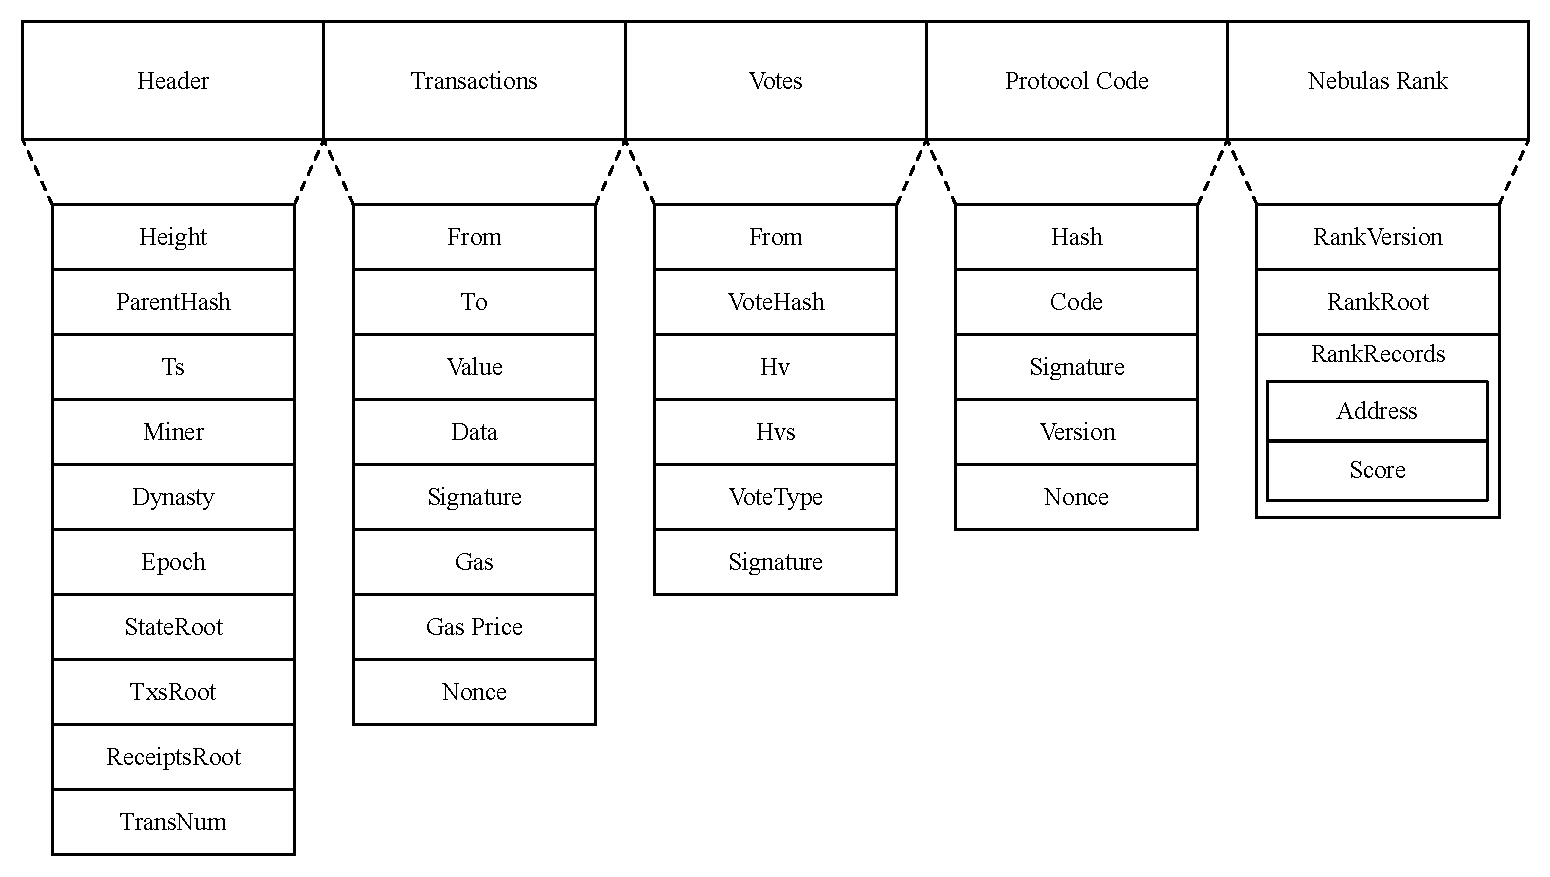
\includegraphics[width=13.8cm]{./figs/block}
\caption{Estructura del bloque}
\label{fig:block}
\end{figure}

De forma similar a otros sistemas de criptodivisa, la interacción entre la cuenta y el blockchain se realiza a través de una transacción en particular. La cuenta crea una transacción, que se firma con una clave privada, la envía a cualquier nodo del blockchain y la transmite al nodo de red completo a través de la red P2P. Durante el intervalo fijo del tiempo de bloque, los nodos especificados por el algoritmo de consenso PoD (ver \refsec{sec:pod}) recogen todas las transacciones en ese lapso, las empaquetan en bloques de formato estándar y las transmiten al resto de la red. Una vez verificado por cada nodo, el nuevo bloque se añade al blockchain local y luego pasa a formar parte del blockchain global.

En Ethereum, las transacciones están divididas en dos tipos: transacciones de cuentas ordinarias y transacciones de contratos inteligentes. En nuestro caso, añadimos dos tipos de transacción nuevos a nuestros bloques: código de protocolo y Nebulas Rank. El código de protocolo, como parte de los datos en el blockchain, se almacenan allí, y la actualización del protocolo básico de Nebulas se lleva a cabo mediante la inserción de datos adicionales en el blockchain. Basado en el algoritmo de valuación NR, el valor NR de cada cuenta se calcula una vez por ciclo y se almacena en el blockchain correspondiente para facilitar la llamada a valores NR en tiempo real, y para realizar consultas históricas.

\subsubsection{Actualización del código del protocolo}

El nodo cliente de Nebulas puede obtener el bytecode compilado de la máquina virtual (NVM bytecode) desde el área de almacenamiento del código de protocolo en el último bloque creado. Si no hay datos del mismo en ese último bloque, significa que el código de protocolo no tiene ninguna actualización, y se debe buscar la versión actual en el bloque más cercano.

Cualquier acción sobre los blockchains será determinada por el código de protocolo, incluyendo el algoritmo de autenticación, las reglas de empaquetado, el algoritmo NR, el mecanismo de incentivos, etc. Casi todas las acciones de los blockchains pueden ser definidas por el código de protocolo.

Si el código del protocolo necesita ser actualizado, el equipo de desarrollo de Nebulas será responsable de su desarrollo y el código será liberado para abrir canales de discusión y votación en las comunidades. La votación se puede llevar a cabo en forma de contrato inteligente o de votación en el foro. Si la mayoría de los miembros de la comunidad están de acuerdo en actualizar el protocolo, el equipo de desarrollo de Nebulas empaquetará el último código en la transacción de código de protocolo, y lo liberará a todos los nodos de la red; una vez que los nodos de contabilidad lo incluyan en bloques, será válido a la altura del bloque especificado. Este tipo de actualización del protocolo en el blockchain es transparente para los clientes sin necesidad de recurrir a \textit{forks}.

Para asegurarse que el código de protocolo se libere después de la autorización, el responsable de su publicación debe utilizar la dirección reservada para el núcleo de Nebulas, que no es modificable en el bloque génesis. Todos los nodos de contabilidad verificarán la firma del código de protocolo. Si la firma no supera la verificación, se considerará que se trata de datos ilegítimos.

La medida de mejora subsiguiente es cambiar la verificación de la firma del código de protocolo por el sistema multifirma M-de-N, que se puede implementar mediante la misma actualización del código de protocolo. %TRADUCIDO
\subsection{Actualización del diseño de los contratos inteligentes}

\subsubsection{Lenguaje de programación Turing-completo de contratos inteligentes}

Un contrato inteligente es un conjunto de \textit{promesas} definidas de forma digital, lo que incluye acuerdos de contrato para la ejecución de esas promesas por parte de los participantes. Físicamente, el soporte del contrato inteligente es un código informático que una computadora puede reconocer y operar. El lenguaje de scripting de Bitcoin es imperativo y basado en pila, por lo que es Turing-incompleto y sus aplicaciones son limitadas. Ethereum es el primer caso en el mundo de un sistema blockchain que implementa contratos inteligentes Turing-completos; adopta Solidity y Serpent como lenguajes, lo que les permite a sus desarrolladores escribir una amplia variedad de aplicaciones de forma rápida y sencilla. Una vez que el código de un contrato inteligente se publica es posible ejecutarlo automáticamente sin intervención de ningún organismo.

En sus primeras etapas, el lenguaje de programación de contratos inteligentes de Nebulas era totalmente compatible con Solidity, lo que facilitaba a los desarrolladores la migración de sus aplicaciones de Ethereum a Nebulas. Añadimos a nuestra implementación de Solidity un conjunto de instrucciones específicas relacionadas a Nebulas Rank con el fin de facilitarles a los desarrolladores la obtención de la valuación NR de cualquier usuario. Luego, basándonos en nuestra NVM, comenzamos a brindar soporte a varios lenguajes de programación, como Java, Python, Go, JavaScript, Scala, etc., con el fin de que cualquier desarrollador familiarizado con ellos tenga la posibilidad de escribir su propio contrato inteligente o DApp.

\subsubsection{Contratos actualizables}

Actualmente, al diseñar un contrato inteligente en Ethereum, no es posible cambiar el código una vez que se ha implementado en la red. En un principio los contratos inteligentes servían como un acuerdo propiamente dicho, por lo cual era razonable entender el diseño como inmutable una vez implementado; el problema está en que, si los desarrolladores no prueban debidamente el código, una vez implementado, será imposible actualizar su código.

No obstante, a medida que los contratos inteligentes se popularizaron, su flujo de trabajo y su código se hicieron cada vez más complicados. En cuanto un hacker encuentra un error, es muy difícil prevenir las pérdidas. En junio de 2016 ocurrió el famoso ataque DAO, producto de un error en el código, lo que causó una pérdida total de \$60 millones de dólares entre los usuarios de Ethereum. A eso debe sumársele un error en la cartera \textit{Parity} que también resultó en la pérdida de 150 000 ETH, valuados en ese momento en \$30 millones de dólares. Debido a que Bitcoin fue diseñado como un sistema Turing-incompleto y muchas de las instrucciones de scripting no están disponibles, su nivel de seguridad es muy alto.

Aunque existen muchas buenas prácticas en la programación de contratos inteligentes, procesos de revisión estrictos e incluso herramientas de verificación formal para asegurar el buen funcionamiento del contrato inteligente a través de pruebas matemáticas, nunca será posible afirmar que un código está totalmente libres de errores. Cuando observamos la historia de Internet, encontramos que para todos los errores graves siempre hubo una actualización disponible en breve. Por ello, creemos que el requisito fundamental para resolver el problema de seguridad de los contratos inteligentes es formular para ellos una solución de diseño actualizable.

Existen dos soluciones propuestas al problema de la inmutabilidad de los contratos inteligentes en Ethereum: la primera es permitir que el Proxy Contract esté disponible al público. Su código es muy sencillo: sólo se encarga de reenviar las peticiones al verdadero contrato inteligente. Cuando se requiere una actualización del contrato inteligente, sólo es necesario hacer que el puntero del \textit{Proxy Contract} apunte al nuevo contrato. La segunda es hacer que el código y el almacenamiento del contrato queden separados. El almacenamiento es responsable de proveer al contrato externo de métodos de lectura y escritura para el estado interno; el código del contrato es responsable de la lógica real, y al llevarse a cabo una actualización, sólo es responsable de implementar el nuevo código del contrato, de modo de no perder el estado actual. Las dos soluciones tienen sus propias limitaciones, por lo que no pueden resolver todos los problemas. Por ejemplo, la separación del código y el almacenamiento hace que el desarrollo de contratos inteligentes sea más complejo, tanto que en ocasiones resulta imposible. Aún cuando el \textit{Proxy Contract} es capaz de apuntar a los nuevos contratos, los datos de estado del contrato anterior no se pueden migrar; a su vez, algunos contratos no fueron bien diseñados en la primera etapa de desarrollo, por lo que no podrán adaptarse para este mecanismo de actualizaciones.

En nuestro caso, diseñamos una solución sencilla al problema de la actualización de contratos que consiste en que, a nivel de lenguaje, cualquier otro contrato con las credenciales adecuadas puede leer y escribir directamente en las variables de estado. Por ejemplo, para un contrato de \textit{tokens} cuyo código se muestra en la figura \ref{figure:nf:oldsc}. \\

	\begin{figure}[!h]
  	\centering
  	\begin{minipage}{0.95\linewidth}
	\begin{lstlisting}[frame=single]
contract Token {
  mapping (address => uint256) balances shared;

  function transfer(address _to, uint256 _value) returns (bool success) {
     if (balances[msg.sender] >= _value) {
       balances[msg.sender] -= _value;
       balances[_to] += _value;
       return true;
     } else {
       return false;
     }
   }
   function balanceOf(address _owner) constant returns (uint256 balance) {
       return balances[_owner];
   }
}
	\end{lstlisting}
  	\end{minipage}
  	\caption{Código de contrato original}
  	\label{figure:nf:oldsc}
	\end{figure}

Al implementar el contrato, las variables de tipo balance se marcan con la palabra clave \texttt{shared}, y al compilarlo como bytecode, la máquina virtual crea un área de almacenamiento separada para este tipo de variables. Las variables que no están marcadas como \texttt{shared} no pueden ser leídas directamente por otros contratos.

Si existe un error en la función de transferencia del código original y es necesario modificarlo, se debe chequear la variable \_value e implementar el nuevo código del contrato inteligente tal como se muestra en la figura \ref{figure:nf:newsc}.

	\begin{figure}[!h]
  	\centering
  	\begin{minipage}{0.95\linewidth}
	\begin{lstlisting}[frame=single]
[baseContractAddress="0x5d65d971895edc438f465c17db6992698a52318d"]
//baseContractAddress is the address of the old contract
contract Token {
  mapping (address => uint256) balances shared;

  function transfer(address _to, uint256 _value) returns (bool success) {
     if (balances[msg.sender] >= _value ^&& _value > 0^) {
       balances[msg.sender] -= _value;
       balances[_to] += _value;
       return true;
     } else {
       return false;
     }
   }
   function balanceOf(address _owner) constant returns (uint256 balance) {
       return balances[_owner];
   }
}
	\end{lstlisting}
  	\end{minipage}
  	\caption{Nuevo código de contrato}
  	\label{figure:nf:newsc}
	\end{figure}

Luego de implementar el nuevo contrato, el anterior se puede autodestruir —lo que significa que ya no será posible acceder al mismo—, pero todas las variables \textit{shared} se mantendrán intactas. El nuevo contrato puede heredar por completo los balances del viejo contrato sin perder ningún estado, por lo que no se requiere ningún paso adicional en la migración. No obstante ello, al desarrollar un contrato inteligente, es necesario declarar explícitamente las variables críticas de estado como \textit{shared}. El compilador manejará especialmente el área de almacenamiento de esas variables de modo de asegurar que sean accesibles a cualquier otro contrato autorizado.

Para garantizar la seguridad, el nuevo contrato debe provenir del mismo creador que el contrato original; de no ocurrir así, surgirá una excepción durante la operación, que no podrá completarse.

Existe un problema moral con este sistema: una vez que un contrato se ha propuesto, se han tomado en recaudo todas las previsiones, se ha escrito y se ha finalizado, el mismo no debería sufrir más modificaciones, y en caso de requerirse alguna corrección técnica (por un error en el código, por ejemplo), esa modificación debería someterse a la decisión de una audiencia. Por ello, planeamos implementar un mecanismo de voto para aprobar la actualización de todo contrato inteligente, impidiendo así que sus autores realicen modificaciones sobre el mismo sin dar aviso a sus usuarios.

Con esta solución para las actualizaciones, el ataque DAO o el error de paridad —o cualquier ataque o error similar— podrán ser corregidos de forma mucho más rápida, sin necesidad de recurrir a ningún \textit{fork}. Luego de aplicar la actualización, los activos de todos los usuarios podrán seguir utilizándose sin necesidad de realizar ninguna migración. %TRADUCIDO
\newpage
\section{Protocolo de Incentivos para Desarrolladores (\textit{Developer Incentive Protocol}, DIP)}
\label{sec:dip}

\subsection{Metas de diseño}
\label{dip:design}

Con el fin de crear una comunidad atractiva en Nebulas proponemos la puesta en servicio del Protocolo de Incentivos para Desarrolladores (DIP) —destinado a programadores de contratos inteligentes en Nebulas— que recompensa con NAS a los más destacados.

\subsection{Algoritmo de distribución de recompensas}
\label{dip:arith}

Creemos que un buen contrato inteligente depende de la cantidad de usuarios que están dispuestos a usarlo. A mayor cantidad de cuentas con buena valuación, mejor será el contrato inteligente. Se utiliza Nebulas Rank a modo de criterio de valuación universal de dichas cuentas. El diseño de DIP combina NR y el concepto común de WAA (\textit{Weekly Active Addresses}, o Direcciones Activas Semanalmente), y el valor WAA total obtenido se utiliza para la valuación del contrato inteligente.

El cómputo del DIP se realiza semanalmente. Para un contrato inteligente \textit{C}, asumimos que el conjunto de direcciones de cuenta activas de esa semana es WAA (\textit{Weekly Active Acounts}). Según la valuación NR en \refsec{subsec:leaderrank} (se toman las diez principales), la suma de los valores NR de las direcciones activas esa semana se calcula como el SCS (\textit{Smart Contracts Score}, o Puntaje de Contratos Inteligentes) del Contrato C, tal como se muestra en la ecuación \ref{formula:dip:scs}.

\begin{align}
\label{formula:dip:scs}
SCS(C)=\sum_{addr \in WAA}(max\{X + 1 - NR(addr), 0\})
\end{align}

Con base en el cómputo semanal de SCS (Puntaje de Contratos Inteligentes), las recompensas se clasifican de mayor a menor de acuerdo a su SCR (\textit{Smart Contract Rank}, Valuación de Contratos Inteligentes). Se toman los mejores $N$ contratos inteligentes, de las cuales sus desarrolladores compartirán $M$ NAS en concepto de recompensas, y en forma proporcional al SCR. Con el fin de evitar manipulaciones en la clasificación, la curva de distribución DIP está diseñada para ser uniforme como se muestra en \reffig{fig:dipdis}, pero aún así se asegura que los ingresos de la valuación 1 sean 2 veces mayores que los de la valuación $N$ para indicar la diferencia en SCS. Las restricciones de proporción se muestran en la ecuación \ref{formula:dip}.

\begin{alignat}{2}
Coin(C) = & \quad kln(N+1-SCR(C))+b \label{formula:dip} \\
\mbox{s.t.}\quad & kln(N) + b = 2b \nonumber \\
& \sum_{x=1}^{N}(kln(x) + b) = M \nonumber
\end{alignat}

\begin{figure}[h]
\centering
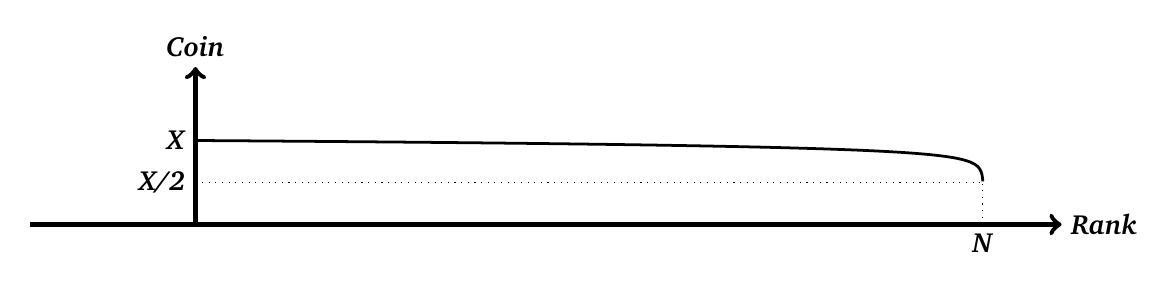
\begin{tikzpicture}
\coordinate (OR) at (0.00, 0.00);
\coordinate (LX) at (-2.10, 0.00); % left x
\coordinate (RX) at (11.00, 0.00); % right x
\coordinate (BY) at (0.00, 0.00); % bottom y
\coordinate (TY) at (0.00, 2.00); % top y
\draw[->][line width=1.75pt] (LX) -- (RX);
\node[right,black] at (11,0) {\textbf{\textit{Rank}}};
\draw[->][line width=1.75pt] (BY) -- (TY);
\node[above,black] at (0, 2) {\textbf{\textit{Coin}}};
\draw[dotted] (0,0.533210267)--(10,0.533210267);
\draw[dotted] (10,0)--(10,0.533210267);
\node[below,black] at (10, 0) {\textbf{\textit{N}}};
\node[left,black] at (0, 0.533210267) {\textbf{\textit{X/2}}};
\node[left,black] at (0, 1.066420536) {\textbf{\textit{X}}};
\draw[black, line width=1.00pt, domain=0:10.00,samples=3000] plot[smooth](\x, {.066598275 * ln(3001-\x * 300) + .533210267});
\end{tikzpicture}
\caption{Curva de distribución de recompensas DIP}
\label{fig:dipdis}
\end{figure}

Las recompensas DIP se calcularán separadamente y serán distribuidas por cada nodo. Asumiendo que un bloque dado se genera cada S segundos (s), las recompensas DIP se calcularán una vez cada 24*7*3600/S bloques para todos los nodos, y serán distribuidas a las direcciones de retiros de los contratos inteligentes.

Con el fin de fomentar la diversidad de los contratos inteligentes de Nebulas y estimular buenos resultados por parte de más desarrolladores, DIP estipula que cada contrato inteligente puede ser recompensado hasta K tiempo(s). DIP seleccionará los mejores $N$ contratos inteligentes cualificados para recibir recompensas de acuerdo a su valuación, con el fin de promover el desarrollo de la construcción de aplicaciones blockchain en el ecosistema.

\subsection{Resultados experimentales}
\label{dip:economic}

Recopilamos los datos de las transacciones realizadas en mayo de 2017 en la red Ethereum y calculamos la clasificación DIP de la primera semana, como se muestra en la tabla \ref{table:dip}.

\begin{table}[h]
\centering
\begin{threeparttable}[b]
\caption{Los mejores 10 resultados de la valuación DIP de la primera semana de mayo de 2017\tnote{1}}
\label{table:dip}
\begin{tabular}{ccc} \toprule
    {Dirección del contrato} & {Puntuación} & {Descripción\tnote{2}} \\ \midrule
0xa74476443119a942de498590fe1f2454d7d4ac0d & 264456363.0 & GolemToken \\
0x49edf201c1e139282643d5e7c6fb0c7219ad1db7 & 207900181.0 & TokenCard-ICO \\
0x48c80f1f4d53d5951e5d5438b54cba84f29f32a5 & 129625776.0 & REP-Augur-OLD \\
0x6810e776880c02933d47db1b9fc05908e5386b96 & 108324489.0 & Gnosis-TokenContract \\
0x6090a6e47849629b7245dfa1ca21d94cd15878ef & 54429341.0 & ENS-Registrar \\
0x607f4c5bb672230e8672085532f7e901544a7375 & 48526808.0 & RLC \\
0x8d12a197cb00d4747a1fe03395095ce2a5cc6819 & 46498412.0 & etherdelta\_2 \\
0xf7b098298f7c69fc14610bf71d5e02c60792894c & 43746158.0 & GUPToken \\
0xaaaf91d9b90df800df4f55c205fd6989c977e73a & 42026627.0 & TokenCardContract \\
0xaec2e87e0a235266d9c5adc9deb4b2e29b54d009 & 41427314.0 & singularDTVToken \\
\bottomrule
\end{tabular}
\begin{tablenotes}
  \small
  \item[1] rango de los bloques: [3629091, 3665815]
  \item[2] datos tomados de etherscan.io
\end{tablenotes}
\end{threeparttable}
\end{table}

Se puede ver que los contratos de mayor rango son más visibles y activos en el ciclo de cálculo, lo que está en línea con nuestra intención original de motivar a los constructores del ecosistema.

\subsection{Análisis de fraudes}
\label{dip:sybil}

Los contratos inteligentes sólo se pueden llamar de forma pasiva. En consecuencia, si un estafador desea incrementar la valuación de su contrato inteligente, tendrá que encontrar cuentas con una valuación NR lo suficientemente altas que realicen llamadas a su contrato.

En primer lugar, será imposible para los estafadores mejorar su clasificación DIP de forma gratuita. Se asume que ellos buscarán mejorar su posición en el Contrato C mediante la creación de un gran número de cuentas para ello. Sin embargo, cuando el SCS se calcula en la ecuación \ref{formula:dip:scs}, sólo los $N$ mejores SCS en el ranking NR obtendrán una valuación mayor a 0, mientras que el ranking NR de las nuevas cuentas estará fuera de esa clasificación. Incluso si realiza llamadas al Contrato C desde las cuentas, no habrá ningún impacto en la valuación DIP.

En segundo lugar, si el estafador está dispuesto a pagar una cierta suma para mejorar la valuación DIP de su contrato, tiene sólo dos alternativas su alcance. La primera de ellas es crear cuentas con una valuación NR alta y realizar llamadas al Contrato C por su cuenta. Este escenario ha sido analizado para la creación de cuentas con alta valuación NR en \refsec{subsec:robust}. Para mejorar la valuación NR en cada una de sus cuentas —mediante la alteración de su topología— necesitará una gran cantidad de dinero. Más allá de eso, debido a que NR se actualiza periódicamente, le resultará muy costoso mantener alta su valuación NR. La segunda alternativa es encontrar un gran número de cuentas cuya valuación NR sea alta, y persuadir o sobornar a sus propietarios para que realicen llamadas al Contrato C. Esta acción, sin embargo, es muy difícil de llevar a cabo a gran escala. Lo que es peor, aquellas cuentas con alto valor NR representarán únicamente un pequeño porcentaje de las mejores $N$, lo que representará, globalmente, un impacto casi nulo en contratos legítimamente sobresalientes. %TRADUCIDO
\newpage
\section{El algoritmo de consenso Prueba de Devoción (\textit{Proof of Devotion}, PoD)}
\label{sec:pod}

\subsection{Metas de diseño}
\label{pod:goals}

La consolidación de los algoritmos de consenso es uno de los hitos más importantes de los blockchains, y su celeridad e irreversibilidad son nuestro norte. Además, con el fin de construir un buen ecosistema en Nebulas, creemos que la equidad es tan importante como los factores ya mencionados. Si cualquier actor con un gran capital puede ganar fácilmente una posición dominante con el fin de controlar el consenso de los bloques en Nebulas, los intereses de los desarrolladores y los usuarios se verán gravemente afectados. Es difícil crear valor añadido en un ecosistema que no puede garantizar los intereses de sus contribuyentes, y esto es algo que va contra los principios de diseño de nuestra plataforma. Por esto, el algoritmo de consenso debe estar diseñado de tal manera que garantice en primer lugar la celeridad y la irreversibilidad del blockchain, para luego buscar la equidad tanto como sea posible, de modo de garantizar los intereses de nuestros contribuyentes.

\subsection{Defectos de los algoritmos de consenso comúnmente utilizados}
\label{pod:weakness}

Hemos intentado encontrar algoritmos de consenso conocidos y apropiados que coincidieran con nuestras metas de diseño, pero ninguno de ellos cubría todas nuestras necesidades.

El algoritmo PoW (Prueba de Trabajo, o \textit{Proof of Work} en inglés) es un juego de suma cero que hace uso de una competencia en el cálculo de hashes para determinar quién tendrá el rol de \textit{contador} que generará nuevos bloques, desperdiciando una gran cantidad de energía eléctrica en ello, y haciendo así que el costo del \textit{minado} sea alto y que la velocidad de generación se vea restringida. Con el aumento de la cantidad de nodos involucrados en minería, las chances que cada nodo tiene de obtener \textit{derechos de contaduría} se ven reducidos, llevando a un incremento sostenido en los costos de generación de bloques bajo este protocolo. Bitcoin, que continúa incrementando la \textit{dificultad de minado}, tendrá que enfrentarse tarde o temprano a la situación inevitable en la que los mineros no podrán hacer frente a los costos; por otro lado, Ethereum ha considerado durante mucho tiempo el uso del sistema de consenso PoS que provee el algoritmo Casper \cite{casper} para reemplazar gradualmente el consenso PoW que usa actualmente \cite{buterin2013ethereum}. Se puede ver que, dado el costo del minado y su velocidad, el algoritmo PoW no es benéfico en el largo plazo para el desarrollo del ecosistema de Nebulas, algo que va contra nuestra meta de celeridad.

El algoritmo de consenso PoS (Prueba de Participación, o \textit{Proof of Stake} en inglés) busca utilizar el depósito de activos en garantía como reemplazo del poder de cálculo de hashes, y distribuye la probabilidada de obtener derechos de contaduría de acuerdo al monto depositado por cada candidato, o la antigüedad de esos depósitos. En la actualidad, tanto Peercoin \cite{king2012peercoin} como el protocolo Casper (en proceso de adopción por Ethereum) implementan el consenso PoS. Este algoritmo supera la deficiencia del alto consumo de energía de PoW pero aumenta visiblemente el impacto del capital en la distribución de la probabilidad de lograr derechos de contaduría. Comparado con PoW, cualquier capital de consideración, bajo PoS, tiene más chances de obtener el poder de controlar el ecosistema, y de formar un monopolio (u oligopolios), dañando así los intereses de los contribuyentes, e impactando de forma negativa en la generación de valor de Nebulas. Todo ello va en oposición a nuestra meta de equidad.

El consenso llamado PoI (Prueba de Importancia, o \textit{Proof of Importance} en inglés) fue propuesto originalmente por Nem \cite{nem}. A diferencia de PoS, este algoritmo introduce el concepto de importancia de las cuentas, cuya valuación se utiliza para la distribución de las probabilidades de obtener derechos de contaduría. Este algoritmo supera la deficiencia del alto consumo de energía de PoW y alivia la vulnerabilidad de PoS con respecto a los monopolios, pero expone un nuevo problema, llamado \textit{nada en juego}\footnote{\textit{Nothing at stake} en inglés, es decir, que nada se ha puesto en garantía (N. del T.)}. Para un estafador, el costo de revertir un bloque se reduce significativamente, lo que va contra nuestra meta de irreversibilidad.

En resumen: en vista de la discrepancia entre nuestras metas y los algoritmos de consenso utilizados comúnmente, hemos propuesto un nuevo sistema llamado PoD (Prueba de Devoción, o \textit{Proof of Devotion} en inglés) que integra las características de PoI —que evalúa la influencia integral de la cuenta— y las de PoS —que lleva aparejadas estrictas sanciones económicas—. PoS mejora la irreversibilidad ofrecida por PoI, mientras que PoI elimina la posibilidad de la existencia de monopolios (posibles en PoS), todo lo cual facilita el desarrollo rápido y libre del ecosistema.

\subsection{Diseño del algoritmo PoD}
\label{pod:design}

\subsubsection{Generación de nuevos bloques}
\label{pod:design:block}

De forma similar a como el algoritmo de consenso PoI selecciona cuentas de alta importancia, PoD selecciona las que poseen una alta influencia en el ecosistema; la diferencia entre ellas radica en que PoD selecciona de forma equiprobable las cuentas que participarán del sorteo a los derechos a la contaduría (generación de nuevos bloques), lo cual impide la posibilidad de la formación de monopolios.

Utilizamos NR —el sistema de valuación de Nebulas— para la selección de cuentas de gran influencia. En el diseño de ese algoritmo destacamos la liquidez y la propagación de las cuentas (consúltese \refsec{subsec:value} para más detalles). Creemos que las cuentas caracterizadas por esas propiedades tienen una gran influencia con respecto a la construcción del ecosistema. Así, en el sistema PoD, serán seleccionadas las cuentas que ingresan en las \textit{N mejores valuaciones NR}, y luego del pago voluntario de una suma determinada de NAS por parte de los dueños de esas cuentas, calificarán como validadores de nuevos bloques, participando así de la \textit{contaduría}.

Luego de crear el conjunto de cuentas validadoras, el algoritmo PoD utiliza su generador de números pseudoaleatorios para determinar cuál de las cuentas en el conjunto será la encargada de empaquetar las transacciones recientes para almacenarlas en un nuevo bloque. El conjunto de validadores es mutable, y las cuentas seleccionadas puede elegir permanecer en él o no. Al margen de ello, las cuentas seleccionadas podrán variar de acuerdo al cambio periódico de la lista NR.

% I removed this sentence as it's a tautology, a redundant statement.
%Therefore, we designed the dynamic validator set change mechanism in the PoD to implement the change of the validator set.

\subsubsection{Conjunto dinámico de validadores}
\label{pod:design:validators}

El conjunto de validadores se modifica al mismo tiempo que lo hacen las dinastías, por lo que cada conjunto de validadores se divide en diferentes dinastías, y cada conjunto dentro de una dinastía permanece inmutable. Las dinastías sólo admiten cambios tras un periodo de tiempo mínimo determinado. Así, se define una Época como el tiempo de duración de X bloques, y dentro de una misma Época, no deben ocurrir cambios de dinastías. Para decirlo de otro modo, los cambios de dinastías sólo podrán ocurrir cuando ocurra un \textit{cambio de Época}. En ese instante se analizará el primer bloque de la Época anterior; si ese bloque alcanza el estado de \textit{finalidad}, la Época actual entrará en la siguiente dinastía de D1; si no, se mantendrá la dinastía previa (D0); el proceso se muestra en la \reffig{fig:epoch}.

\begin{figure}[h]
\centering
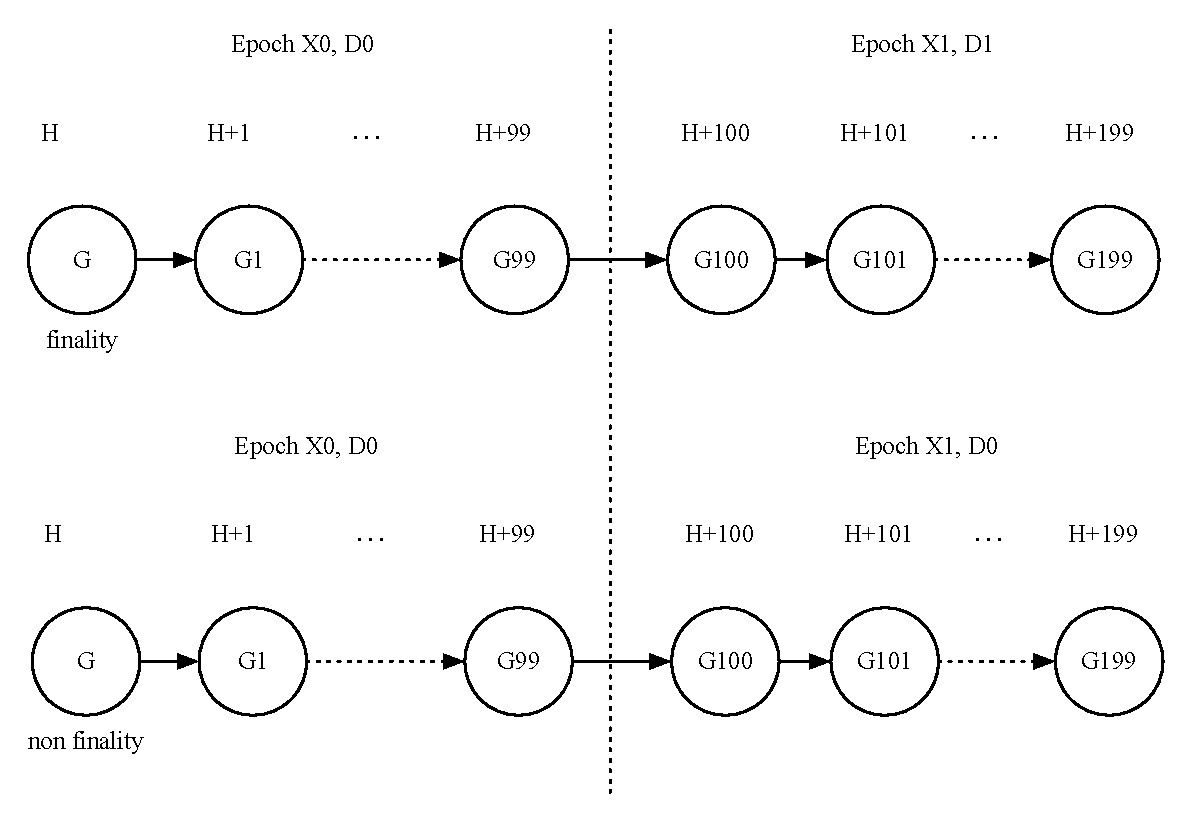
\includegraphics[width=10cm]{./figs/epoch}
\caption{Cambio de dinastías de validadores (asumiendo X = 100)}
\label{fig:epoch}
\end{figure}

A causa de las demoras en la red, el estado de finalidad del bloque G en cada uno de los nodos podría no ser el mismo cuando ocurre el cambio de dinastía. Por ello, haciendo referencia al conjunto de estrategias del validador dinámico Casper, será necesario el proceso de consenso de cada dinastía se complete en forma conjunta al conjunto de validadores de las dinastías previa y actual. Así, en cualquier dinastía, una cuenta elegible sólo podrá aplicar para el enlistamiento (o renuncia) en el conjunto de validadores de la dinastía D+2; así, cuando la dinastía D+2 esté vigente, podrá participar en el proceso de consenso del nuevo bloque.

\subsubsection{Proceso de consenso}
\label{pod:design:consensus}

Luego de que un nuevo bloque es propuesto, todos los participantes del conjunto de validadores de la dinastía actual podrán participar en una ronda de votos tolerante a faltas bizantinas, con el fin de determinar la legitimidad del bloque. Al comienzo de la votación, a cada validador que participe del consenso del bloque se le cobrará 2x (x es la proporción del bono incentivo) como depósito; a partir de ese momento se iniciará el proceso de votación en dos etapas que se describe a continuación:

\begin{itemize}

\item \textbf{En la primera etapa} será necesario que todos los validadores emitan el ticket de voto $Prepare$ por el nuevo bloque. Luego de emitir el ticket de voto $Prepare$, el validador recibirá un bono de $1.5x$. Si los validadores que poseen más de dos tercios del total de los depósitos tanto en la dinastía previa como la actual emiten los tickets de voto $Prepare$ por el nuevo bloque, ese bloque entrará en la segunda etapa de votación. Nótese que el propositor del nuevo bloque emite por defecto un ticket de voto $Prepare$ por el nuevo bloque.

\item \textbf{En la segunda etapa} se requiere que todos los validadores emitan tickets de voto $Commit$ para el nuevo bloque. Luego de la emisión de $Commit$, los validadores recibirán otro bono de $1.5x$. Si los validadores que poseen más de dos tercios del total de los depósitos tanto en la dinastía previa como la actual emiten los tickets de voto $Commit$ por el nuevo bloque, el mismo alcanzará el estado de finalidad.
\end{itemize}

Para acelerar el desarrollo del ecosistema, si la diferencia entre el timestamp de $Prepare$ y $Commit$ en el bloque $b$ y el timestamp del bloque $b$ excede $T$, esos tickets se considerarán expirados y se ignorarán.

\subsubsection{Elección de \textit{forks}}
\label{pod:design:fork}

El algoritmo PoD selecciona la cadena canónica de acuerdo al puntaje del bloque en cada \textit{altura}\footnote{\textit{Height} en inglés (N. del T.)}. Se seleccionará siempre el bloque que posea el mayor puntaje para unirse a la cadena canónica. El puntaje del bloque $b$ en la altura $h$ se calcula de este modo:

\begin{align}
Score(b, h) = \sum_{(b',h') \in children(b)}Score(b', h') + \sum committed~deposits~in~b
\end{align}
\noindent

Es decir, es la suma de los depósitos recibidos por este bloque y todos sus descendientes, correspondientes al ticket $Commit$, tal como se muestra en la \reffig{fig:fork_choice}.

\begin{figure}[h]
\centering
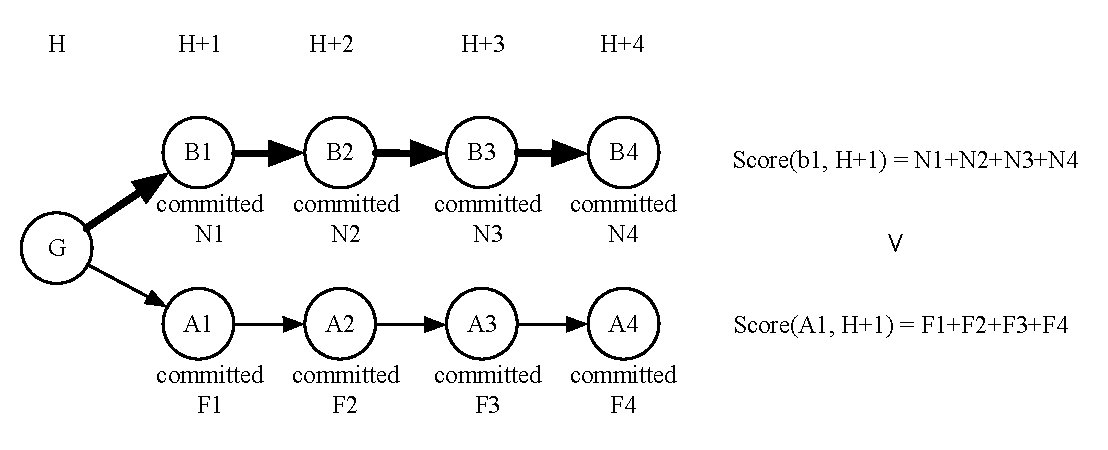
\includegraphics[width=12cm]{./figs/fork}
\caption{Fork Choice Example}
\label{fig:fork_choice}
\end{figure}

\subsubsection{Condiciones de confiscación}
\label{pod:design:vote}

Para evitar cualquier daño malicioso al proceso de consenso —que puede dar lugar a un fracaso en la finalización del proceso de consenso y a una obstrucción del desarrollo del ecosistema— PoD restringe las actividades de consenso de los validadores basándose en las condiciones mínimas de confiscación de Casper \cite{minimal_slash_rules}.

Asúmase que los tickets de voto $Prepare$ y $Commit$ en el proceso de consenso tienen la estructura siguiente:

\begin{itemize}
\item $Prepare(H, v, vs)$, donde $H$ es el valor hash del bloque actual; $v$ representa la altura del bloque actual; $vs$ representa la altura de un determinado bloque ancestral de $v$.

\item $Commit(H, v)$, donde $H$ es el valor hash del bloque actual; $v$ representa la altura del bloque actual.
\end{itemize}

El algoritmo PoD define las siguientes cuatro reglas básicas para el proceso completo de votación:

\begin{itemize}
\item Existe un orden estricto en el proceso de consenso de dos etapas de un bloque: sólo será posible para los validadores emitir los tickets de voto $Commit(H, v)$ de la segunda etapa cuando los depósitos totales de los tickets de voto $Prepare(H, v, vs)$ de la primera etapa alcanzan $2/3$.

\item Para bloques múltiples, no existen reglas que obliguen a esperar a que finalice un proceso de consenso antes de iniciar el siguiente. El consenso entrelazado está permitido siempre y cuando se lleve a cabo en cierto orden; sólo después de que la primera etapa de votación esté completa y la proporción de tickets de voto $Prepare(H, vs, vs’)$ alcance $2/3$ se podrán enviar los tickets $Prepare(H, v, vs)$ para los bloques descendientes, para asegurar la estabilidad de esta modalidad de consenso.

\item Para evitar que un nodo cualquiera pueda realizar votaciones interbloque maliciosas tomando ventaja del \textit{consenso entrelazado}, se requiere que luego de enviados los votos (H, w, u) basados en la altura de u, ningún voto Commit(H, v) se pueda enviar a aquellos bloques con una altura dentro del rango que va de $u$ a $w$, garantizando así la eficiencia y el orden en el proceso de consenso.

\item Con el fin de prevenir que los nodos puedan realizar el depósito de caución\footnote{\textit{Staking} en inglés (N. del T.)} en distintas ramas al mismo tiempo —lo que podría generar el problema de \textit{nada en juego}— se requiere que luego de emitir los votos $Prepare(H1, v, vs1)$ en una altura determinada, no sea posible emitir otro voto $Prepare(H2, v, vs2)$.
\end{itemize}

Una vez reportado y verificado, todo validador que viole las reglas citadas previamente recibirá una sanción y sus depósitos serán confiscados; de la confiscación, 4\% se repartirán entre quienes hayan reportado el incidente, y el resto será destruido.

\subsection{Análisis económico de la PoD}
\label{pod:economic}

\subsubsection{Análisis de incentivos}
\label{pod:economic:incentive}

Todo validador que participe del algoritmo PoD será recompensado con $1x$ NAS por cada bloque legítimo creado. En caso de no finalizar la etapa $Prepare$ e ingresar en la etapa $Commit$ debido a problemas de tráfico en la red o por comportamientos fraudulentos, el validador perderá $0.5x$ NAS. De ese modo, todo validador obtendrá una suma importante en concepto de ganancias de contaduría siempre y cuando mantenga una buena conexión de red y no se vea envuelto en actividades fraudulentas.

\subsubsection{Análisis de fraudes}
\label{pod:economic:fraud}

\subsubsection*{Ataque de doble gasto}
\label{pod:economic:fraud:double_spend}

Si se asume que un comerciante confirma una transacción y la envía cuando el nuevo bloque alcanza el estado de finalidad, entonces el costo mínimo a pagar por un fraude de compra sin costo por medio de un ataque de doble gasto bajo el consenso PoD se describe de este modo:

Primero, el estafador necesita incrementar su valuación Nebulas Rank para ingresar a los N principales\footnote{\textit{Top N} en inglés (N. del T.}, convertirse en validador mediante el pago de una suma $N$ de NAS como depósito de caución, y aplicar para la participación en la validación de bloques en la dinastía D+2.

Luego, el estafador necesita resultar seleccionado como propositor de un nuevo bloque a través del algoritmo pseudoaleatorio. En ese momento, el estafador propone dos nuevos bloques a la misma altura, de los cuales uno de los bloques tiene un valor hash $hash1$ y contiene una transferencia desde el estafador hacia el comerciante, mientras el otro bloque tiene un valor hash $hash2$ y contiene una transferencia desde el estafador hacia sí mismo.

Finalmente, para lograr que ambos bloques alcancen el estado de finalidad —como se muestra en la  \reffig{fig:double_spend}— el estafador necesita gastar $1/3$ del total de los depósitos en esa dinastía para sobornar a $1/3$ de los validadores y hacer que emitan tickets de voto $Commit$ para ambos bloques.

\begin{figure}[h]
\centering
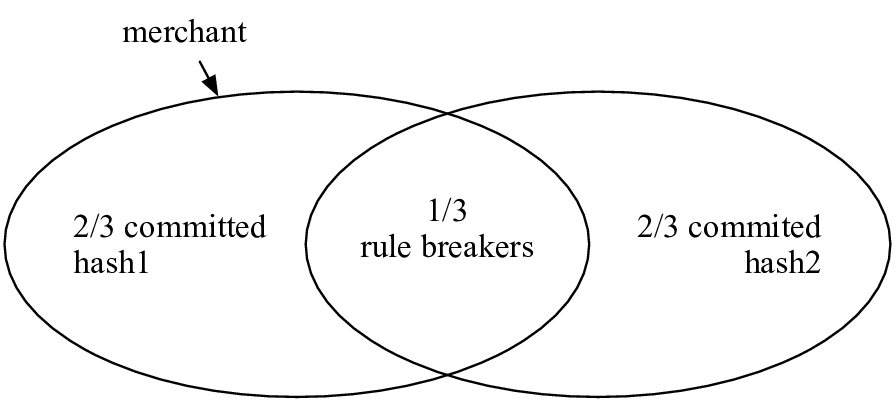
\includegraphics[width=7cm]{./figs/overlap}
\caption{Sanción financiera en casos de doble gasto}
\label{fig:double_spend}
\end{figure}

Por lo tanto, para completar un ataque exitoso de doble gasto, el estafador necesita gastar una determinada cantidad de energía y recursos financieros para incrementar su valuación Nebulas Rank (véase \refsec{subsec:robust}, “resistencia a la manipulación”) y entonces gastar al menos $1/3$ del valor total de los depósitos en esa dinastía para lograr que ambos bloques alcancen el estado de finalidad si es los suficientemente afortunado como para resultar selecto como propositor.

\subsubsection*{Ataque del 51\%}
\label{pod:economic:fraud:51attack}

En el consenso PoW, lanzar un ataque del 51\% implica poseer al menos el 51\% del poder de cómputo de la red entera. En el consenso PoS, es necesario contar con el 51\% del total de depósitos en caución. No obstante, en nuestro consenso PoD, un ataque del 51\% requiere poseer el 51\% de las cuentas del conjunto de validadores, lo que significa que un número significativo de cuentas de reputación necesitan ingresar a los \textit{N principales} de Nebulas Rank y realizar el pago de los depósitos de caución para cada una de las cuentas, por lo que un ataque de estas características es mucho más difícil en el algoritmo de consenso PoD.

\subsubsection*{Ataque de corto alcance}
\label{pod:economic:fraud:short_range_attack}

En PoD, los bloques de cada altura tienen plazo de caducidad para el consenso. Por lo tanto, es casi imposible completar un ataque de largo alcance en PoD, pero aún es posible lanzar ataques de corto alcance dentro del plazo de caducidad.

Si un atacante de corto plazo intenta fraguar la cadena $A$ para reemplazarla por la cadena $B$ con el fin de convertirla en el \textit{fork canónico} cuando los bloques a la altura de $H+1$ todavía se encuentran fuera del tiempo de expiración, necesitará asegurarse de que el puntaje del bloque $A1$ es mayor que el del bloque $B1$. El voto múltiple recibe sanciones muy fuertes, por lo que le resultará inevitable al atacante sobornar a los validadores; de otro modo, es imposible concretar un ataque de este tipo. Con el fin de demostrar la seguridad del algoritmo PoD, se muestran a continuación los costos que debe pagar el atacante para revertir un número dado de bloques.

Si el atacante planea revertir $B1$, el costo mínimo que debe pagar se describe en la  \reffig{fig:revert1}, que equivale al costo de un ataque de doble gasto. Si el atacante se convierte en un propositor de bloques a la altura de $H+1$, deberá sobornar a $1/3$ de los validadores en la dinastía $D0$ y convencerlos de realizar votaciones múltiples para lograr que $A1$ alcance el estado de finalidad, para lo cual el costo mínimo es de $1/3$ del total de los depósitos.

\begin{figure}[h]
\centering
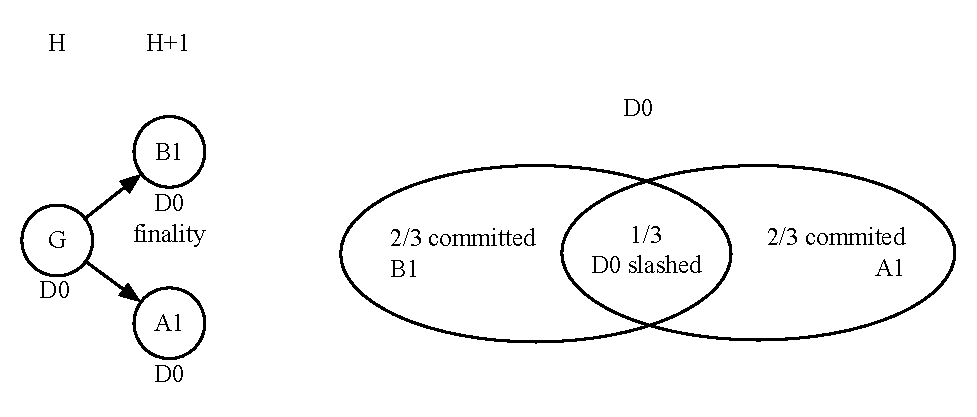
\includegraphics[width=11cm]{./figs/revert1}
\caption{Reversión de un bloque por parte de un atacante de corto plazo}
\label{fig:revert1}
\end{figure}

Asumiendo que $B1$ y $B2$ alcanzaron el estado de finalidad y las transacciones en los bloques han surtido efecto, si el atacante desea revertir $B1-B2$, se toman las dos circunstancias siguientes en consideración:

\begin{itemize}
\item La primera circunstancia se muestra en la \reffig{fig:revert2} (a): cuando las alturas $H+1$ y $H+2$ se encuentran en la misma época y dinastía, el atacante necesita sobornar a $1/3$ de los validadores en D0 para lograr que $A1$ alcance el estado de finalidad. Mientras tanto, ese $1/3$ de los validadores recibirán sanciones y sus depósitos serán totalmente confiscados. Durante la validación de $A2$, la suma de los depósitos equivale a $2/3$ de los depósitos en $A1$. En ese momento, si el atacante desea asegurar la misma cantidad de votos que en $B2$, debe sobornar al resto de los validadores sin cometer fraude, y perder al menos $3/3$ de los depósitos totales. Incluso en el caso de que el atacante tenga éxito en hacer esto, es imposible garantizar que el puntaje de $A1$ sea mayor que el de $B1$, con lo que el atacante enfrentará una alta probabilidad de fallar en el ataque.

\item La segunda circunstancia se muestra en la \reffig{fig:revert2} (b): cuando las alturas $H+1$ y $H+2$ están en distintas épocas y dinastías, el atacante necesita sobornar a $1/3$ de los validadores en $D0$ para lograr que $A1$ alcance estado de finalidad, y luego sobornar a $1/3$ de los validadores en $D1$ para lograr que $A2$ alcance también estado de finalidad, por lo que el atacante deberá perder al menos $2/3$ de los depósitos totales con el fin de completar tal ataque. En suma, para lanzar un ataque de corto plazo para causar la invalidación de dos bloques que han alcanzado el estado de finalidad, el atacante necesita pagar al menos $2/3$ de los depósitos totales.
\end{itemize}

\begin{figure}[h]
\centering
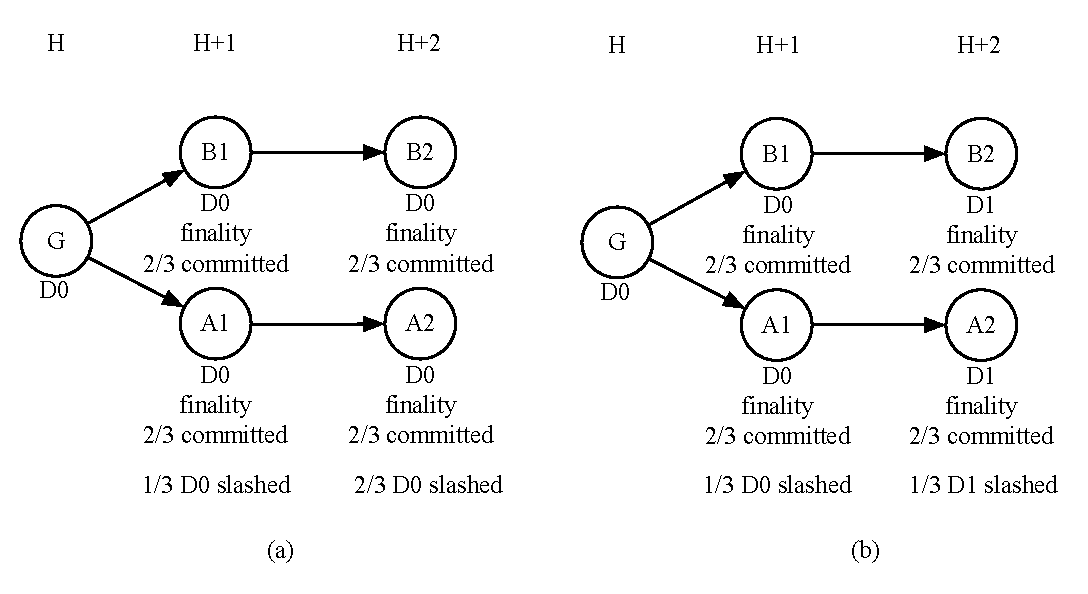
\includegraphics[width=11cm]{./figs/revert2}
\caption{Reversión de dos bloques mediante un ataque de corto plazo}
\label{fig:revert2}
\end{figure}

Si el atacante desea revertir $B1-B3$, como se muestra en la \reffig{fig:revert3}, necesitará primero sobornar a $1/3$ de los validadores en D0 para alcanzar la finalidad de $A1$ y luego sobornar a $1/3$ de los validadores de la dinastía $D1$ para alcanzar la finalidad de $A2$. Finalmente, el atacante necesita sobornar a los $2/3$ de los validadores en $D1$ para lograr la finalidad de $A3$. Resumiendo, perderá $4/3$ de los depósitos totales. Le resultará muy difícil preparar un ataque de estas características. Incluso si logra éxito en sus preparaciones, no puede garantizar que el puntaje de $A1$ sea mayor que el de $B1$. Por lo tanto, es muy probable que un ataque tal falle.

\begin{figure}[h]
\centering
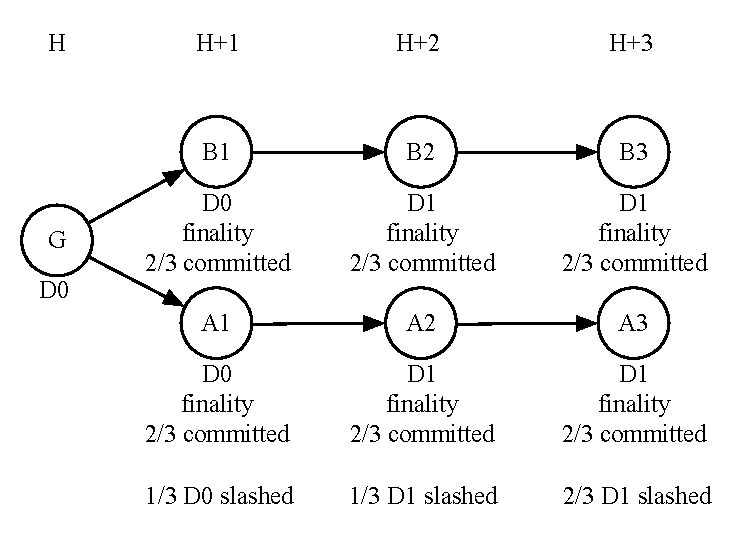
\includegraphics[width=7.5cm]{./figs/revert3}
\caption{Reversión de tres bloques mediante un ataque de corto plazo}
\label{fig:revert3}
\end{figure}

En general: si un atacante desea revertir $B1-BN$ —en donde $N$ está limitado por el plazo de vencimiento del consenso del bloque y por ende no puede ser un número muy grande— cuando $N = 3$, el total de los depósitos de todos los validadores de la dinastía actual serán completamente confiscados. Así, cuando $N >= 4$, será imposible completar el ataque para lograr que el puntaje de $B1$ sea mayor que $A1$ y así revertir $B1-BN$. No tendría sentido alguno un ataque de estas características. %TRADUCIDO
\newpage
\section{Motor de búsquedas en el blockchain}
\label{sec:search}

\subsection{Introducción}

A medida que los desarrolladores implementan una cantidad cada vez más creciente de contratos inteligentes, se acrecienta la necesidad de contar con una herramienta nativa de búsqueda de contratos inteligentes. Dado que éstos son básicamente código y que no incluyen ninguna descripción de su funcionalidad, su indexación por medio de las tecnologías de motores de búsqueda existentes impone una enorme dificultad.

Con el fin de indexar correctamente los contratos inteligentes, hacemos uso de los siguientes métodos:

\begin{itemize}
	\item Rastreo de datos en páginas web relevantes a los contratos inteligentes con el fin de establecer mapeos entre los datos y los contratos inteligentes del blockchain.

	\item Alentar a los desarrolladores a cargar contratos inteligentes cuyo código fuente ha sido verificado exhaustivamente; analizar las funciones y la semántica del código, crear índices para el mismo, y brindar funciones de búsqueda para contratos similares. Descompilar aquellos contratos inteligentes que no cuentan con código fuente.

	\item Establecer estándares para los contratos inteligentes, de modo que cualquier contrato que coincida con ellos pueda ser hallado por los usuarios. Además, alentar a los desarrolladores a brindar descripciones informativas de los contratos durante su creación. \\

	\begin{figure}[ht]
  	\centering
  	\begin{minipage}{.4\linewidth}
	\begin{lstlisting}[frame=single]
contract SearchableContract {
   string public language;
   string public author;
   string public name;
   string public title;
   string public description;
   string public tags;
}
	\end{lstlisting}
  	\end{minipage}
	\end{figure}

\end{itemize}

\subsection{Infrastructura}

En esta etapa creemos que los motores de búsqueda centralizados son los más adecuados para obtener la mejor experiencia de usuario y para presentar las valuaciones de Nebulas Rank. Nuestro equipo de desarrollo está dedicado a desarrollar un servicio de búsqueda capaz de obtener todos los contratos inteligentes en tiempo real, realizar un análisis multilingüe de sus palabras y crear índices de texto completo con el fin de brindarles a los usuarios una interfaz web amigable.

La veracidad del algoritmo de valuación NR y la verificabilidad de cada nodo aseguran la imparcialidad de un servicio de búsqueda centralizado, siempre que el código completo del \textit{backend} de búsqueda esté disponible a la comunidad. Además, cualquier desarrollador podrá crear su propio servicio de búsqueda sobre esta base.

La \reffig{fig:search-arch} muestra la arquitectura del servicio de búsqueda.

\begin{figure}[h]
\centering
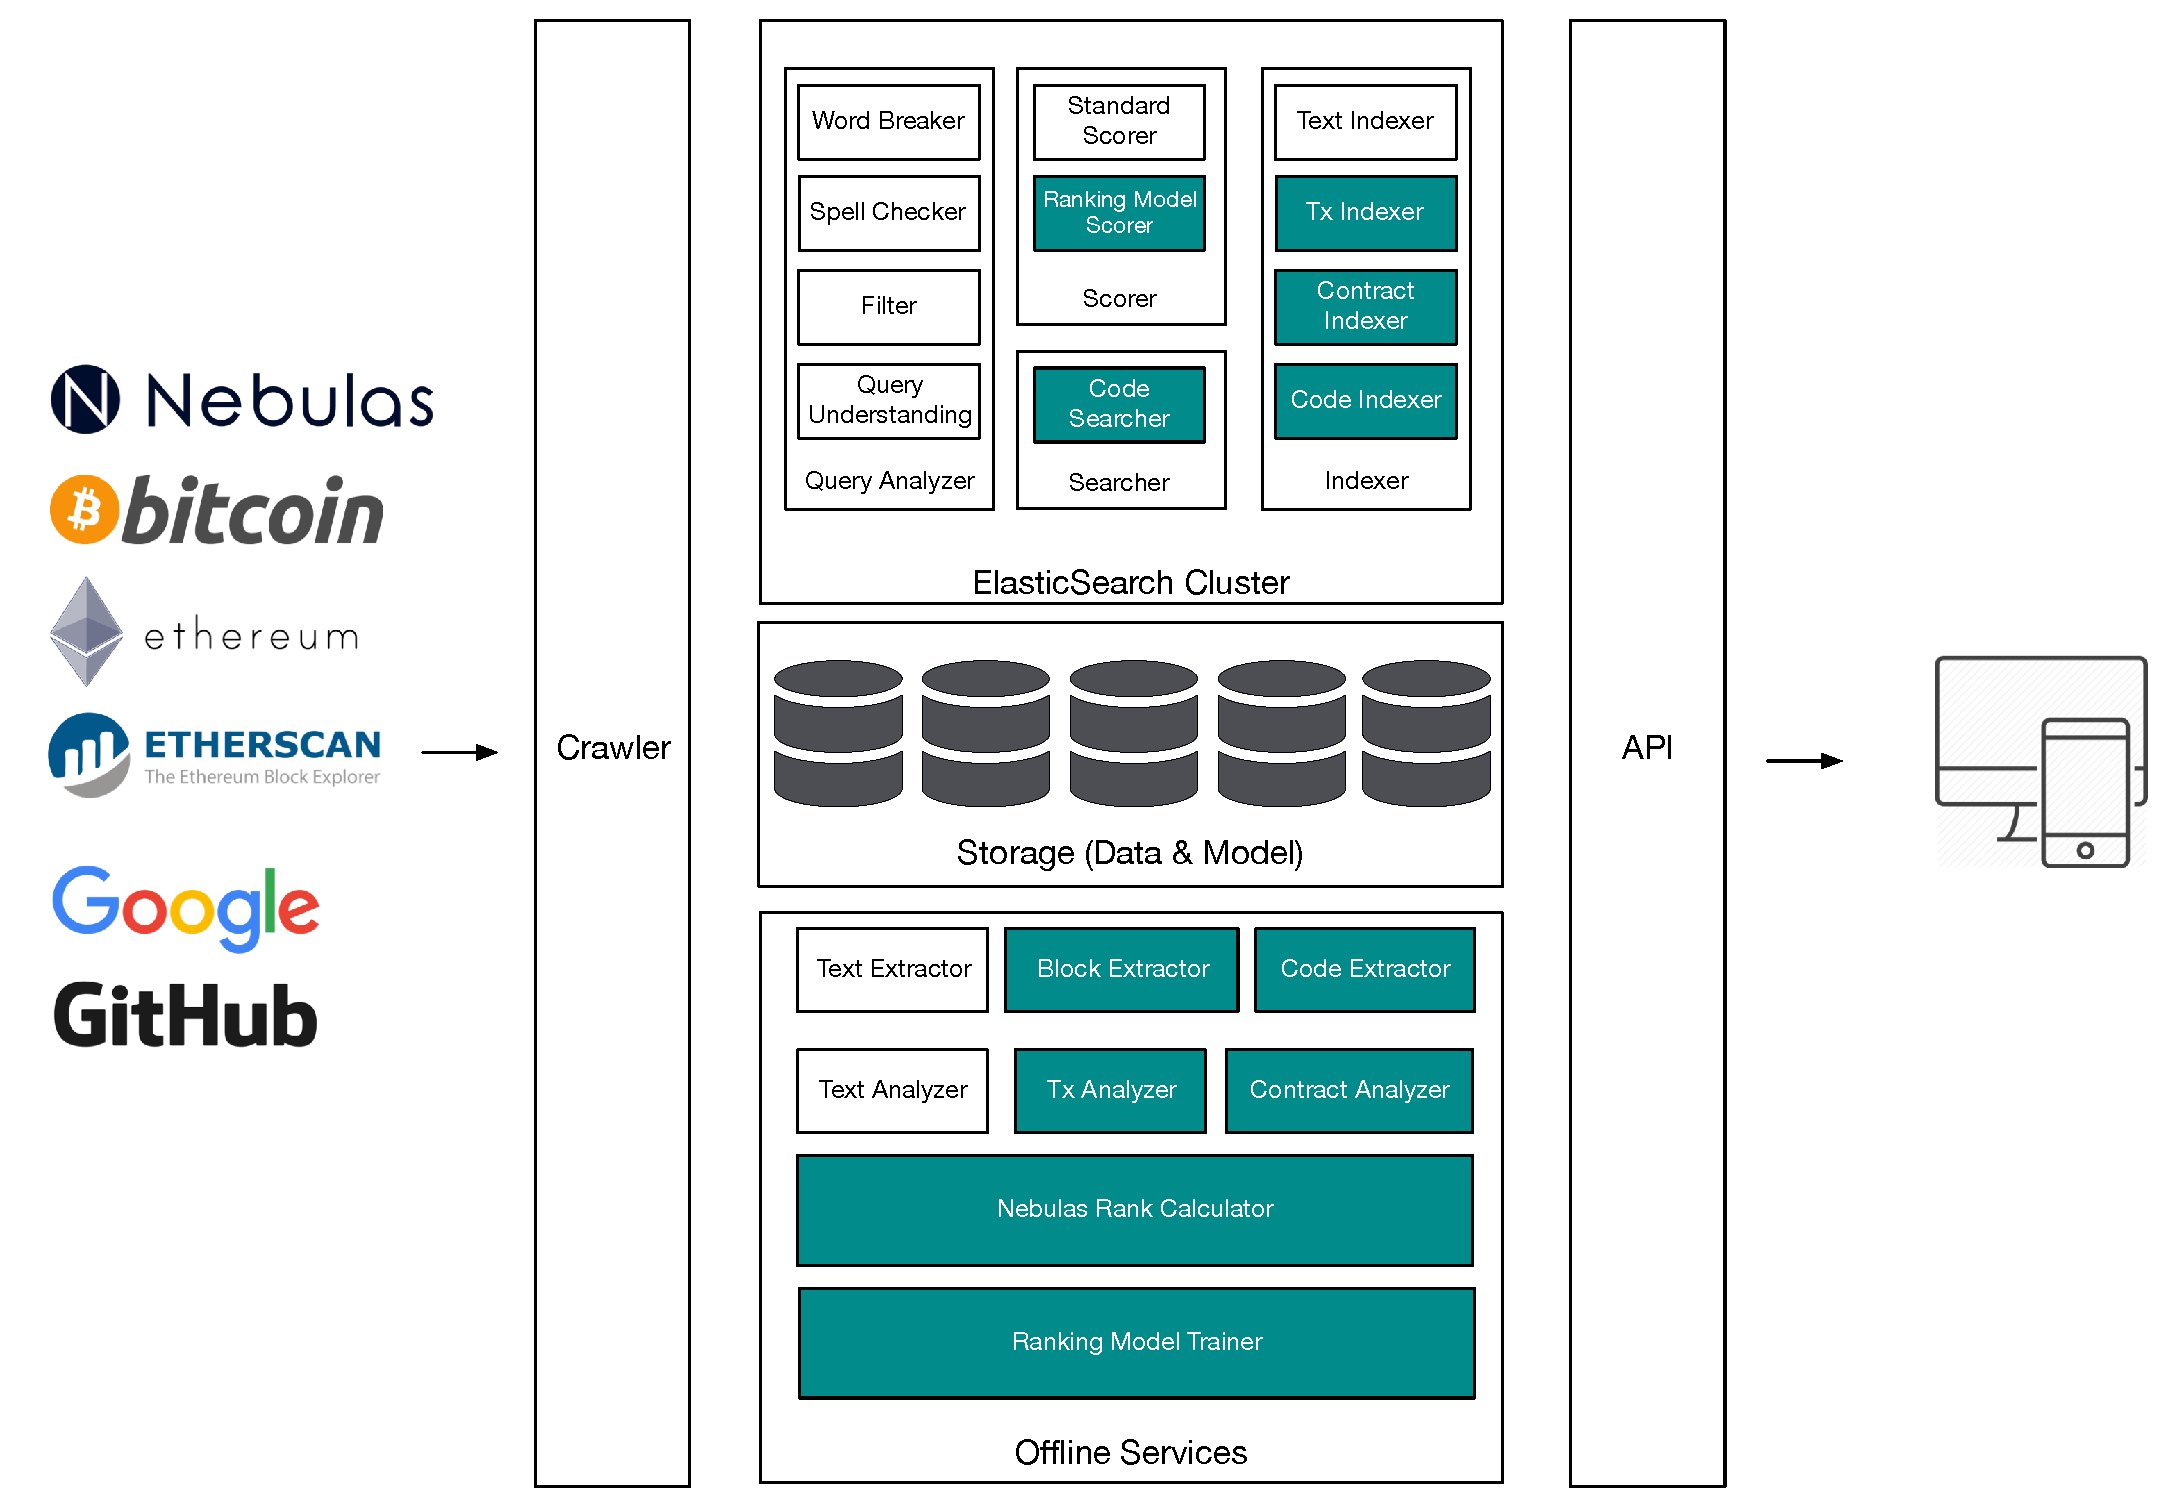
\includegraphics[width=16cm]{./figs/search-arch-new}
\caption{Arquitectura del servicio de búsqueda}
\label{fig:search-arch}
\end{figure}

\begin{itemize}
	\item \textbf{Crawler:} los orígenes de los datos del \textit{crawler} del motor de búsqueda blockchain se clasifican en dos tipos: a) búsqueda de información sobre los bloques y el código de los contratos inteligentes en los blockchains; b) búsqueda de información sobre contratos inteligentes desde URL públicas incluyendo introducciones, comentarios de los usuarios acerca de las Dapps, y noticias relacionadas.

	\item \textbf{Extractor:} consiste del Extractor de Texto, del Extractor de Bloques y del Extractor de Código, los cuales proveen servicios de extracción de textos, bloques y código de contratos inteligentes, respectivamente.

	\item \textbf{Analyzer:} consiste del Analizador de Textos, del Analizador de Transacciones y del Analizador de Contratos, que brindan información sobre textos, información de transacciones en bloques, y análisis de contratos inteligentes, respectivamente. Este último permite descompilar contratos, extraer sus códigos fuente, realizar análisis semánticos, y más.

	\item \textbf{Nebulas Rank Calculator:} se refiere al servicio de cálculo de Nebulas Rank, que se utiliza para computar la valuación NR de cada cuenta, sea de usuarios o contratos.

	\item \textbf{Ranking Model Trainer:} hace referencia al servicio de entrenamiento del modelo de valuación. Las reglas de valuación toman en cuenta múltiples factores: coincidencia de campos, relevancia de textos, valuación NR del contrato, cantidad de transacciones efectuadas por el mismo, frecuencia y profundidad, valuación NR del usuario que efectúa una transacción con el contrato, y la seguridad de éste. Basándose en las condiciones de uso reales del usuario, el algoritmo de aprendizaje (el GBDT y las redes neuronales artificiales, o ANN, son opcionales) se utiliza para entrenar el modelo de valuación y puntuación, que además están en constante mejora de acuerdo al \textit{feedback} del usuario. El modelo entrenado se utiliza luego para el \textit{Scorer} del servicio de búsquedas.

	\item \textbf{Query Analyzer:} se refiere al servicio de análisis de palabras clave, que incluye el sistema multilingüe \textit{Word Breaker} y el corrector ortográfico (\textit{Spell Checker}).

	\item \textbf{Indexer:} se encarga de crear índices apropiados para el Analyzer y da soporte a índices completos e incrementales.

	\item \textbf{Scorer:} se clasifica en dos niveles:
	\begin{itemize}
		\item \textbf{Nivel 1:} \textbf{Standard Scorer} recupera los conjuntos de resultados del candidato de ElasticSearch, lo cual se hace para recuperar tantos resultados de candidatos como sea posible a través de la clasificación eficiente y efectiva en el cluster de ElasticSearch. Este nivel puede recuperar varios miles de resultados.
		\item \textbf{Nivel 2:} \textbf{Ranking Model Scorer} utiliza el modelo de valuación \textit{offline} para calcular y reorganizar la valuación de cada candidato del conjunto de resultados del \textit{nivel 1}. En este nivel, los resultados calculados tienen una precisión abrumadora y pueden ser utilizados directamente por los usuarios.
	\end{itemize}
	\item \textbf{Searcher:} es el responsable de comunicarse con el cluster ElasticSearch y empacar y devolver el resultado de la búsqueda al \textit{frontend}.

	\item \textbf{API:} le proporciona a las aplicaciones externas servicios de búsqueda completos de API.

	\item \textbf{ElasticSearch Cluster:} Se refiere al cluster de servidores. El equipo de desarrollo de Nebulas planea utilizar el motor de búsqueda de código abierto ElasticSearch para dar soporte a la indización de texto completo.

\end{itemize}

\subsection{\textit{Nebulas Trends}}

Este sistema genera, en combinación con Nebulas Rank, la lista de tendencias para brindar valores visuales multidimensionales de usuario en los blockchains.

\begin{itemize}
\item \textbf{Lista Nebulas Rank para direcciones de usuarios:} muestra la lista NR diaria y las listas NR de cambios rápidos en valuaciones ascendentes y descendentes. Además, con esta lista es posible visualizar la tendencia en la variación de la valuación de cada cuenta y la tendencia en los cambios de salud de la red completa.

\item \textbf{Lista Nebulas Rank para cuentas de contratos inteligentes:} basándose en los valores NR de las cuentas de usuarios, se calcula la lista NR de las cuentas de los contratos inteligentes, la lista de cambios rápidos en valuaciones ascendentes y descendentes, la tendencia en la variación de cada contrato y el gráfico de tendencias para la cantidad y la frecuencia de uso de los contratos inteligentes en toda la red. Además, se añadirán las listas de contratos de tokens y la lista de estimación de contratos de mercado para mostrar una dimensión más amplia de la información.

\item \textbf{Lista de desarrolladores de contratos inteligentes:} de acuerdo a lo descripta en el punto anterior, la lista de desarrolladores de contratos inteligentes enumera las contribuciones de éstos y los casos de rápido ascenso en el \textit{ranking} con el fin de mostrar tanto las {\dapp}s sobresalientes como sus desarrolladores.

\end{itemize}

\subsection{Consulta de palabras clave}

Mediante una palabra clave o una descripción textual —tal como su título, su función o su autor— los usuarios podrán encontrar, entre cualquier cantidad de contratos inteligentes, aquellos que coinciden con esos criterios. En este momento se encuentran disponibles varios algoritmos sofisticados y maduros para su búsqueda mediante texto. Al utilizar procesamiento de lenguaje natural y tecnologías de índice inverso, es posible ordenar y recuperar de forma eficiente la información almacenada en bases de datos cargadas masivamente de contratos inteligentes. Para ello, se hace uso de la siguiente tecnología:

\begin{enumerate}
	\item Rastreador distribuido orientado a tópicos.
	\item Segmentación de palabras multilingüe: la segmentación de palabras es una tarea relativamente simple para los lenguajes occidentales; para las palabras chinas, en cambio, se han puesto a disposición los siguientes algoritmos: coincidencia máxima positiva, coincidencia mínima positiva, segmentación por ruta más corta y segmentación estadística.
	\item Corrección de términos de búsqueda y comprensión semántica.
	\item Índice inverso y arquitectura de búsqueda distribuida.
	\item Algoritmo de valuación para ordenar los resultados de la búsqueda.

\end{enumerate}

Entre esas tecnologías, el algoritmo de valuación trabajará en forma combinada con Nebulas Rank. Específicamente, para crear el grafo de transacciones del blockchain utilizamos las transferencias entre usuarios en el mundo blockchain en forma similar a las relaciones de referencias entre los sitios web de internet. Luego, calculamos la valuación NR de las cuentas que no son de contratos inteligentes por medio del uso de la tecnología NR descripta en la sección \refsec{subsec:leaderrank}, calculamos las valuaciones de los contratos por medio del algoritmo descripto en la sección \refsec{dip:arith}, y finalmente utilizamos los resultados para ordenar los resultados de la búsqueda.

\subsection{Búsqueda de resultados similares para contratos inteligentes}

Es de utilidad para los desarrolladores y algunos usuarios la función de búsqueda de contratos inteligentes con funciones similares de acuerdo al fragmento de un código de contrato dado. Al ser diferente de la búsqueda regular de palabras clave, la búsqueda de código similar tiene sus particularidades. Para implementar una función de búsqueda tal, necesitamos hacer uso de un determinado algoritmo capaz de mensurar la similitud del código en porcentajes.

En el mundo académico actual, los algoritmos de similitud de código se clasifican principalmente en distancia de edición de cadenas, similitud de secuencia de tokens, similitud de árboles de sintaxis abstracta y similitud de grafos de dependencias de programas. Estos algoritmos describen la similitud en términos del texto del código, la estructura y la sintaxis, desde diferentes dimensiones. Al combinar esos cuatro algoritmos, planteamos doce características de similitud en el código de los contratos de Nebulas, entre ellas \textit{Skeleton Tree}, signatura y llamadas a librerías. Para más detalles, consúltese el apéndice \ref{appendix:sim_code}.

De forma similar a las búsquedas basadas en palabras clave, los resultados de búsqueda de contratos inteligentes utilizan el mismo algoritmo de valuación de contratos para ordenar los resultados finales. %TRADUCIDO
\newpage
\section{Servicios fundamentales y herramientas de desarrollo}
\label{sec:tools}

\subsection{Servicio de Nombres de Dominio (DNS)}

Debido a la naturaleza anónima de los blockchains, las direcciones de las cuentas son cadenas largas y que no expresan ningún sentido para los humanos, lo que las hace poco amigables con los usuarios, que por este motivo quedan expuestos a perder dinero debido a errores causados por transferencias erróneas, o por interactuar con los objetos equivocados. En otras palabras: al usar nombres de dominio fáciles de recordar, los usuarios se benefician de una mejor experiencia. Por medio del uso de contratos inteligentes, el equipo de desarrollo de Nebulas implementará en el blockchain un sistema similar a DNS, llamado \textit{Nebulas Name Service} (NNS), asegurando que el acceso será irrestricto, gratuito y abierto. Cualquier desarrollador podrá implementar sus propios servicios de resolución de dominio, ya sean independientes o que utilicen NNS.

Para ilustrar la idea: Alicia adquiere el nombre de dominio \textbf{alice.nns} para su dirección\\0xdf4d22611412132d3e9bd322f82e2940674ec1bc03b20e40. Para transferirle dinero a Alicia, Juan sólo necesita memorizar y escribir \textit{alice.nns} en el campo de la dirección de la aplicación NNS para que el dinero le llegue a la persona correcta.

Las reglas para el uso de NNS serán las siguientes:

\begin{itemize}

	\item Los nombres de subdominios de nivel superior quedarán reservados y no estarán disponibles para su contratación; estos nombres incluyen: *.nns, *.com, *.org and *.edu. Los usuarios sólo podrán aplicar a nombres de subdominio de segundo nivel.
	\item Una vez que el servicio NNS esté activo, los usuarios serán capaces de consultar la disponibilidad de los nombres de dominio; de encontrar uno vacante, dichos usuarios podrán ofertar por él a través de un contrato inteligente. El proceso de subasta será abierto, por lo que cualquier usuario podrá consultar la oferta vigente y mejorarla.
	\item Una vez que la subasta termine, el mejor postor ganará el nombre de dominio y el contrato inteligente bloqueará los fondos del oferente. El periodo de validez del nombre de dominio es de un año. Pasado ese plazo, el usuario será libre de renovarlo. De hacerlo, el periodo de validez se extenderá por otro año. Si decide no renovarlo, los fondos de la subasta le serán devueltos al postor y el nombre de dominio quedará disponible nuevamente.
	\item Los usuarios podrán ceder los derechos de un nombre de dominio en cualquier momento. En ese caso, los fondos de la oferta serán devueltos de forma automática a la cuenta del usuario depositante, y el nombre de dominio quedará disponible nuevamente.
	\item Los usuarios podrán transferir la propiedad del nombre de dominio, con o sin compensación. Nebulas no intervendrá en ninguna transacción de nombres de dominio.

\end{itemize}

\subsection{La red Lightning}

En la actualidad todas las redes públicas de blockchain enfrentan desafíos relacionados a la escalabilidad de sus sistemas. Por ejemplo, la red Bitcoin sólo es capaz de procesar siete transacciones por segundo, mientras que Ethereum apenas duplica ese valor, con 15 TPS. Con la introducción de algoritmos de consenso basados en PoS (\textit{Proof of Stake}, o Prueba de Participación), es posible evitar por completo los complejos cálculos del consenso PoW, con lo cual la velocidad de las transacciones se incrementa notablemente. No obstante, los blockchains públicos siguen presentando problemas serios antes escenarios de micropagos en el mundo real. En febrero de 2015 se diseñó la red Lightning \cite{poon2015bitcoin} con el fin de crear un canal dedicado a los micropagos entre distintos actores, de modo de lograr que una gran cantidad de pagos pudieran ser confirmados fuera del blockchain de forma directa, repetida y bidireccionalmente, en un método llamado “de compensación”: cuando es necesario liquidar una serie de transacciones, el resultado final se envía a los blockchains para su confirmación. Teóricamente, esto permite alcanzar millones de transferencias por segundo. Si no existe un canal de pago punto a punto entre las partes, también puede utilizarse una vía de pago que conecte a ambas y que consista en múltiples canales de pago para lograr una transferencia fiable de fondos entre ellas. La red Lightning ya ha demostrado ser útil, y superó la etapa de prueba de concepto tanto para Bitcoin como para Ethereum.

Nebulas implementa la red Lightning como infraestructura de blockchains, ofreciendo así un diseño flexible. Cualquier desarrollador externo puede usar el servicio básico de esta red para desarrollar aplicaciones para escenarios de transacciones frecuentes en Nebulas. En paralelo a esto, Nebulas lanzará la primera cartera del mundo con soporte a esta red.

\subsection{Herramientas de desarrollo}

Es crítico contar con un conjunto de herramientas de desarrollo para la creación de aplicaciones en el blockchain. Hasta el momento, este tipo de herramientas son incompletas, imponiendo grandes retos a la mayoría de los desarrolladores. El equipo de desarrollo de Nebulas proveerá un amplio conjunto de herramientas de desarrollo que incluirá un entorno IDE para contratos inteligentes, un explorador de bloques, \textit{plugins} para los IDE más populares (como Eclipse, JetBrains, Visual Studio, Sublime Text, VIM, y Atom), depuradores, simuladores, herramientas de verificación formal para contratos inteligentes, SDKs para distintos lenguajes y para entornos móviles. %TRADUCIDO
\newpage
\section{Criptodivisa Nebulas (NAS)}
\label{sec:nascoin}

La red Nebulas posee su propia criptodivisa, cuya denominación es NAS. Ésta juega dos roles en la red: primero, como su criptodivisa original, proporciona liquidez de activos entre los usuarios, y funciona como el medio para el cobro de los incentivos para contadores (PoD) y desarrolladores (DIP); segundo, se utilizará esta criptodivisa para el cálculo de las comisiones por ejecución de contratos inteligentes.

La unidad mínima de NAS es $10^{-18}$ NAS.

Originalmente, NAS se distribuyó como un \textit{token} ERC20 en la plataforma Ethereum, con un total máximo agregado de $X = 10^8.$ Los modos de emisión son los siguientes:

\begin{enumerate}
	\item \textbf{Construcción comunitaria:}
	Bajo la dirección del equipo auspiciante de Nebulas, se utilizarán $80\%X$ \textit{tokens} para la construcción de la comunidad de Nebulas, incluyendo la incubación ecológica y los incentivos de la \dapp \textit{Nebulas community blockchain}, la construcción de la comunidad de desarrolladores, la cooperación de industrias y negocios, marketing y promoción, investigación académica, inversión en educación, leyes y regulaciones, e inversiones en comunidades y organizaciones. Específicamente, se venderán $5\%X$ NAS a distintos inversionistas de impacto comunitario, $5\%X$ NAS como fondo de desarrollo comunitario de Nebulas y $70\%X$ NAS se mantendrán como reserva.

	\item \textbf{Incentivos para patrocinadores y equipos de desarrollo:}
	A lo largo del desarrollo de Nebulas, el patrocinador y los equipos de desarrollo realizarán contribuciones continuas de materiales y recursos humanos en aspectos relacionados a la estructura organizativa del proyecto, investigación, desarrollo tecnológico y operación ecológica. En cuanto a la asignación de \textit{tokens}, se reservan $20\%X$ NAS como incentivos para el equipo. Esta parte se bloqueará inicialmente, y se desbloqueará un año después de la finalización de la primera venta de NAS a la comunidad, distribuyéndose gradualmente a los equipos de patrocinadores y de desarrollo a lo largo de tres años.

\end{enumerate}

Luego del lanzamiento oficial de la red Nebulas, cualquier usuario con tokens NAS ERC20 podrá cambiarlos por la criptodivisa nativa de la red Nebulas (también llamada NAS) usando para ello las credenciales relacionadas. A medida que la red Nebulas evolucione, NAS crecerá de la siguiente manera:

\begin{enumerate}
	\item \textbf{Incentivos PoD:} $3\%X$ NAS de incentivos por año para los \textit{contadores};

	\item \textbf{Incentivos DIP:} $1\%X$ NAS de incentivos por año para los desarrolladores destacados de contratos inteligentes.

\end{enumerate} %TRADUCIDO
\newpage
\section{Conclusión}
\label{sec:conclusion}

\subsubsection*{Nuestra postura}

Desde una perspectiva altamente abstracta, un blockchain es \textbf{una forma descentralizada de determinar los datos}, y sus tokens funcionan como \textbf{el soporte para esa determinación}. Mientras Internet resuelve la necesidad de la transmisión de datos, Blockchain va más allá, y resuelve la determinación de esos datos. Por primera vez en la historia, Blockchain convierte los datos públicos en datos privados que ya no serán analizados y utilizados arbitrariamente por grandes empresas como Google, Amazon y Facebook.

La esencia de este nuevo paradigma —representada por los blockchains públicos— es la conjunción de tres elementos: \textbf{comunidad, token, y aplicación}. La \textbf{comunidad} es, esencialmente, un ecosistema construido de abajo hacia arriba, que adhiere a la idea de apertura, código abierto, intercambio y no lucratividad, que es completamente diferente de los ecosistemas empresariales construidos de arriba hacia abajo. El \textbf{token} es el portador del valor de los datos; en el futuro habrá más escenarios de uso para los blockchains que los de moneda virtual y efectivo electrónico. La \textbf{aplicación} se refiere simplemente a la implementación tecnológica de los escenarios de aplicación de los blockchains. Sin la combinación de los dos primeros factores mencionados, una aplicación por sí sola no puede reflejar completamente el atractivo de los sistemas blockchain.

Los atributos de los blockchains públicos (\textbf{veracidad y transparencia}) representan el valor real de estos sistemas. Por el contrario, la mayoría de los blockchains de empresas y consorcios son permisionados o privados, lo que significa que no pueden romper los patrones existentes, y son consideradas como meras innovaciones mejoradas, mientras que los blockchains públicos anulan las relaciones de confianza existentes y se consideran como \textbf{innovaciones revolucionarias}, que reflejan el valor máximo de los blockchains.

\subsubsection*{Nuestro compromiso}

Al ser el primer motor de búsqueda en blockchains del mundo, Nebulas está comprometido a \textbf{explorar las dimensiones ocultas del valor} y en crear sistemas operativos en el blockchain basados en valor, motores de búsqueda y otras aplicaciones relacionadas.

Con este compromiso presentamos \textbf{Nebulas Rank}, un estándar de valuación del mundo blockchain; diseñamos \textbf{Nebulas Force} para implementar la capacidad auto-evolutiva en los blockchains; desarrollamos los sistemas \textbf{Developer Incentive Protocol} y \textbf{Proof of Devotion} para motivar la actualización del valor de los blockchains; y construimos \textbf{Nebulas Search Engine} para ayudar a nuestros usuarios a explorar otras dimensiones en el valor de los blockchains.

\subsubsection*{Nuestras creencias}

La continua evolución científica y tecnológica nos llevará a una vida mejor con un mayor nivel de \textbf{libertad e igualdad}. Como una de las principales tecnologías de nuestro tiempo, los blockchains gradualmente nos mostrarán todo el brillo de sus ventajas. Ser parte de esta evolución es nuestra mayor felicidad y logro.

Al igual que en Internet, los blockchains también entrarán en una fase explosiva en cuanto a cantidad de usuarios y aplicaciones. La tecnología del blockchain se convertirá en el \textbf{protocolo central} de la próxima generación de la red inteligente, y el número de usuarios alcanzará o incluso superará los mil millones en los próximos 5 a 10 años. En los próximos cinco años surgirán importantes oportunidades y desafíos.

Frente al vasto ecosistema del futuro, no nos debemos preguntar qué puede hacer blockchain por nosotros, sino qué podemos hacer nosotros por blockchain, porque \textbf{los blockchains son a la vez un organismo y una economía}.

Estamos encantados de compartir con todos ustedes la exploración de las tecnologías blockchain. %TRADUCIDO
\bibliography{reference} %SIN MODIFICAR

\begin{appendices}
\section{Diseño de las direcciones de cuentas Nebulas}

El diseño de las direcciones de cuentas Nebulas tuvo especial cuidado en colocar la letra \textbf{\textit{n}} como carácter inicial —a modo de inicial para el nombre del proyecto, \textit{Nebulas}.

\subsection{Direcciones de cuentas}

En forma similar a Bitcoin and Ethereum, Nebulas también adopta un algoritmo criptográfico de curva elíptica para sus cuentas. La dirección se deriva de la clave pública, que a su vez se deriva de la clave privada, encriptada con la contraseña del usuario.

El diseño del \textit{checksum} también apunta a evitar que los usuarios envíen NAS de forma accidental a una cuenta equivocada debido a uno o más caracteres escritos incorrectamente.

El método específico de cálculo es el que se provee aquí debajo:

\begin{verbatim}
content = ripemd160(sha3_256(public key))
checksum = sha3_256(0x19<<(21*8) + 0x57<<(20*8) + content)[0:4]
address = base58(0x19<<(25*8) + 0x57<<(24*8) + content<<(4*8) + checksum)
\end{verbatim}

\noindent en donde 0x19 se utiliza como relleno, y 0x57 especifica el tipo de dirección. Nótese que la longitud de \texttt{content} es de 20 bytes, la longitud de \texttt{checksum} es de 4 bytes, y la longitud de \texttt{address} es de 26 bytes.

Una dirección Nebulas contiene un total de 35 caracteres incluyendo el prefijo \textit{n}, y se codifica utilizando el algoritmo base58. Una dirección típica se verá así: \texttt{n1TV3sU6jyzR4rJ1D7jCAmtVGSntJagXZHC}.

\subsection{Direcciones de contratos inteligentes}
El cálculo de las direcciones de los contratos inteligentes difiere ligeramente del utilizado en el párrafo anterior, ya que no se requiere la contraseña, pero sí el \textit{nonce} y la dirección de quien lo implementa. La fórmula es la siguiente:

\begin{verbatim}
content = ripemd160(sha3_256(tx.from, tx.nonce))
checksum = sha3_256(0x19<<(21*8) + 0x58<<(20*8) + content)[0:4]
address = base58(0x19<<(25*8) + 0x58<<(24*8) + content<<(4*8) + checksum)
\end{verbatim}

\noindent
en donde 0x58 indica que la dirección es de un contrato inteligente. Una dirección de este tipo se verá así: \texttt{n1sLnoc7j57YfzAVP8tJ3yK5a2i56QrTDdK}. %TRADUCIDO
\section{Búsqueda de contratos inteligentes similares}
\label{appendix:sim_code}

La dificultad en la búsqueda de similaridad de código radica en las características estructurales de los lenguajes de alto nivel, y en la diversidad de las expresiones lógicas de los contratos inteligentes. En la actualidad existen varias escuelas de algoritmos de búsqueda de similaridad de código en los círculos académicos, las que se describen de este modo:

\begin{itemize}
	\item \textbf{Distancia de edición entre cadenas de caracteres} \\
	Tanto la consulta de código como el código fuente candidato se consideran como texto. La distancia de edición entre dos cadenas de caracteres se utiliza para medir las similitudes entre ambos. La \textit{distancia de edición} se refiere al número mínimo ded operaciones de edición necesarias para convertir una cadena de caracteres en otra. Las operaciones de edición permitidas incluyen la sustitución de un carácter por otro —borrado de un carácter e inserción de otro—. Generalmente hablando, a menor distancia de edición, mayor la similitud entre dos cadenas de caracteres. Este algoritmo basado en distancias de edición entre cadenas de caracteres puede ser usado no sólo para la comparación de códigos fuente sino también en representaciones intermedias o incluso código de máquina.
	Con el fin de mejorar la robustez de estos algoritmos, se llevará a cabo un cierto grado de conversión del código fuente sin introducir cambios semánticos: esto puede ser la remoción de caracteres en blanco, la remoción de comentarios, el reemplazo de los nombres de todas las variables locales con ‘\$’, la normalización de las expresiones algebraicas, etcétera. Este tipo de algoritmos se caracterizan por ser veloces, concisos y muy eficientes. No obstante, su adaptabilidad a programas complejos es relativamente pobre y no tienen en cuenta la sintaxis y la estructura organizativa del código.

	\item \textbf{Secuencia de tokens} \\
	El método de representación de secuencias de tokens se refiere a la conversión del código fuente ingresado en una secuencia de tokens a través del análisis léxico. La similitud entre dos programas se puede ver como la similitud entre dos secuencias de tokens, de modo que se puede utilizar la mayor subcadena en común o un algoritmo de coincidencia de correlación (algoritmo de coincidencia de árboles de sufijos) para medir el grado de similitud entre dos programas, a través del cual se pueden detectar segmentos de código con diferentes sintaxis pero con funciones similares. Sin embargo, este método oculta la estructura organizativa de los programas al medir la similitud entre ellos.

	\item \textbf{Árbol de sintaxis abstracta (\textit{Abstract Syntax Tree}, o AST)} \\
	AST es una forma de expresión intermedia después de realizar un análisis sintáctico en un código fuente, sobre el cual se puede medir la similitud entre dos programas a través de la comparación entre un subárbol y otro. Para medir la similitud entre dos árboles se puede utilizar el algoritmo de distancia de edición de árbol \cite{zhang1989simple}. El algoritmo preciso de la distancia de edición del árbol es relativamente complejo y la literatura al respecto (\cite{guha2002approximate}) proporciona un algoritmo rápido aproximado. De acuerdo a \cite{chilowicz2009syntax}, los árboles de sintaxis deben someterse a una identificación por huella hash con el fin de habilitar al algoritmo de comparación del árbol de sintaxis para realizar búsquedas de alta eficiencia en conjuntos de datos masivos.

	\item \textbf{Grafo de dependencias de programas (\textit{Program Dependency Graph}, o PDG)} \\
	Un PDG \cite{ferrante1987program} puede representar los datos internos, controlar la relación de dependencia de un programa y analizar el código de programa a nivel semántico. Un protocolo de código similar se transforma en una búsqueda de subgrafos isomórficos, que es un problema NP-completo y requiere un algoritmo muy complejo, por lo que sólo algunos algoritmos aproximados están disponibles en la actualidad.

\end{itemize}

Creemos que los algoritmos mencionados describen las similitudes entre códigos en texto, estructura y sintaxis en dimensiones diferentes. Source Forager \cite{kashyap2017source} nos proporciona un gran ejercicio mental: los índices de similitud en distintas dimensiones se representan como características diferentes, cada una de las cuales representa la medición de la similitud del código desde un aspecto específico. Por último, la similitud vectorial se utiliza para llevar a cabo la medición de la similitud general. Este método integra las ventajas de los algoritmos mencionados anteriormente. Esta idea también es utilizada por Nebulas como referencia para realizar la búsqueda de la similitud entre contratos inteligentes. Consideramos que funciona como la unidad fundamental de búsqueda de código entre los contratos inteligentes.

La tabla \ref{table:search-similarity} define las características de similitud entre códigos candidatos. Luego, se describe la definición de cada característica y la función para calcular su similitud:

\begin{table}[h]
\centering
\begin{threeparttable}[b]
\caption{Tabla de familias de características de similitud de código}
\label{table:search-similarity}
\begin{tabular}{ccc} \toprule
    {Clase de características} & {Descripción} \\ \midrule
Emparejamiento tipo-operación & Tipos empleados y operaciones realizadas sobre esos tipos \\
Esqueleto de árbol & Estructura de bucles y condicionales \\
Esqueleto de árbol decorado & Estructura de bucles, condicionales y operaciones \\
BFS sobre 3-grafo del CFG & Subgrafos de un CFG de tamaño 3, usando BFS para generar subgrafos \\
BFS sobre 4-grafo del CFG & Subgrafos de un CFG de tamaño 4, usando BFS para generar subgrafos \\
DFS sobre 3-grafo del CFG & Subgrafos de un CFG de tamaño 3, usando DFS para generar subgrafos \\
DFS sobre 4-grafo del CFG & Subgrafos de un CFG de tamaño 4, usando DFS para generar subgrafos \\
Llamadas a librerías & Llamadas a librerías \\
Signatura & Tipos de entrada y valor devuelto \\
Tipos locales & Tipos de las variables locales \\
Literales numéricos & Constantes de datos numéricos \\
Literal de cadena & Constantes de datos de cadena \\
\bottomrule
\end{tabular}
\end{threeparttable}
\end{table}

\begin{itemize}
	\item \textbf{\textit{Emparejamiento tipo-operación}} \\
	Es un conjunto 2-tupla que contiene el tipo de la variable y su operador, es decir, el par (tipo, operación). Generalmente, los tipos de datos primitivos debe emparejarse con un operador aritmético, un operador lógico y un operador relacional, tal como ($int, \geq$); los tipos de datos personalizados (como las estructuras \texttt{struct}) deben emparejarse con las funciones miembro, tales como (\texttt{Bar}, \texttt{.foo}), indicando que el campo \texttt{foo} del tipo de dato \texttt{Bar} es consultado. Basándonos en esta metodología, todas las operaciones sobre variables en el cuerpo del código de una función se deben transformar en 2-tuplas.

	Después de eliminar repeticiones, se utiliza una secuencia 2-tupla para reflejar la característica de emparejamiento tipo-operación de este segmento de código. Creemos que las piezas de código con funciones similares deben tener similares conjuntos de operaciones sobre variables. No obstante, no nos preocupa el orden de las 2-tuplas, por lo que esta característica pierde la información de la estructura lógica del código y por lo tanto sólo puede representar parcialmente sus características.

	La similitud entre las características de emparejamiento tipo-operación se puede definir mediante similitudes Jacobianas; es decir que dados dos conjuntos $S_1$ y $S_2$, la similitud Jacobiana se puede definir mediante la siguiente fórmula:

	\begin{equation}
	sim_{Jacc(S_{1}, S_{2})}=\frac{\mid S_{1}\bigcap S_{2}\mid}{\mid S_{1}\bigcup S_{2}\mid}
	\end{equation}

	\item Esqueleto de árbol (\textit{Skeleton Tree}) \\
	Árbol de sintaxis abstracta basado en código. Sólo se mantienen las estructuras de bucle (\texttt{for, while, do...while}) y las sentencias condicionales (\texttt{if...else}); todos los otros nodos son removidos del árbol. Creemos que los códigos con funciones similares deberían ser similares en cuanto a estructuras de bucle y sentencias condicionales.

	El cálculo de la similitud para esqueletos de árbol está basado en la distancia de edición entre dos árboles. Se define $d_{r}$ como la distancia de edición estimada entre dos árboles, y está determinada únicamente por el tamaño del árbol, es decir:

	\begin{equation}
	d_{r}(T_{1}, T{2})=\frac{\mid size(T_{1})-size(T_{2})\mid}{max(size(T_{1}), size(T_{2}))}
	\end{equation}

	Se asume $D_T$ como el valor umbral de la distancia de edición, y se fija en 0,5. Podemos adquirir la fórmula para el cálculo de la distancia aproximada de edición entre dos árboles:

	\begin{equation}
	d_{t}(T_{1}, T{2})=\begin{cases}d_{r}(T_{1}, T{2}) & if~d_{r}(T_{1}, T{2})\geq D_{T}\\\frac{max\left(\begin{array}{c}ed(pre(T_{1}),~pre(T_{2})),\\ ed(post(T_{1}),~post(T_{2}))\end{array}\right)}{max(size(T_{1}), size(T_{2}))} & otherwise\end{cases}
	\end{equation}

	$pre(T)$ representa la secuencia transversal del árbol antes de la ordenación; $post(T)$ representa la secuencia transversal del árbol después de la ordenación; $ed(S_{1}, S_{2})$ representa la distancia de edición entre $S_{1}$ y $S_{2}$. La similitud entre dos esqueletos de árbol se puede calcular mediante la siguiente fórmula:

	\begin{equation}
	sim_{Tree}(T_{1}, T{2})=1-d_{t}(T_{1}, T{2})
	\end{equation}

	\item Esqueleto de árbol decorado (\textit{Decorated Skeleton Tree}) \\
	Esta entidad es similar al esqueleto de árbol, aunque además de preservar los nodos de bucle y bifurcación, se conservan la mayoría de los operadores (tales como \texttt{+, -, <}), excepto por \texttt{=} y \texttt{\&}, considerados como \textit{ruido}.

	\item \textbf{K-subgrafos del CFG} \\
	Dado un CFG\footnote{CFG aquí refiere a la locución inglesa \textit{Control Flow Graph}, es decir, grafo de flujo de control (N. del T.)} y un nodo específico, se lleva a cabo una búsqueda BFS\footnote{\textit{Breadth-First Search}, o \textit{búsqueda en anchura} (N. del T.)} o bien una búsqueda DFS\footnote{\textit{Depth-First Search}, o \textit{búsqueda en profundidad} (N. del T.)} hasta que el número de nodos recorridos llegue a $k$, momento en el cual el subgrafo formado debería ser el k-subgrafo. Si el número de nodos no llega a $k$ luego de finalizar el recorrido, dicho subgrafo se debe descartar. Mediante el recorrido de cada nodo en el CFG, podemos adquirir todos los k-subgrafos. Por cada k-subgrafo, es necesario utilizar un entero de $k^2$ bits para expresarlo. Para más detalles, consúltese la \ref{fig:graph-ex}. Todos los k-subgrafos forman un conjunto de enteros.

	\textbf{BFS sobre 3-grafo del CFG:} k = 3, recorrido de árbol BFS

	\textbf{BFS sobre 4-grafo del CFG:} k = 4, recorrido de árbol BFS

	\textbf{DFS sobre 3-grafo del CFG:} k = 3, recorrido de árbol DFS

	\textbf{DFS sobre 4-grafo del CFG:} k = 4, recorrido de árbol DFS

	Dados los vectores $\vec{x}=(x_{1}, x_{2}, ...x_{n})$ y $\vec{y}=(y_{1}, y_{2}, ...y_{n})$, la similitud Jacobiana generalizada se puede definir como:

	\begin{equation}
	J(\vec{x}, \vec{y})=\frac{\sum_imin(x_{i}, y_{i})}{\sum_imax(x_{i}, y_{i})}
	\end{equation}

	\begin{figure}[h]
	\centering
	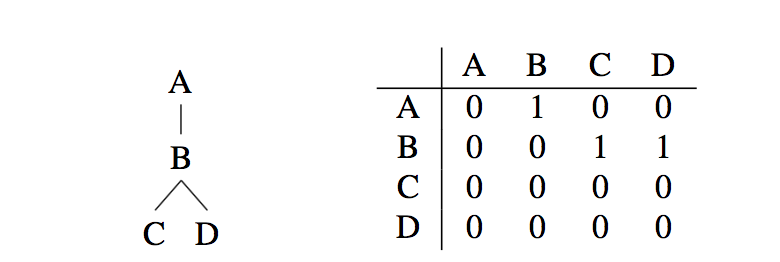
\includegraphics[width=6cm]{./figs/graph-matrix.png}
	\caption{Ejemplo para un 4-grafo: el elemento de la matriz es la cadena binaria \texttt{0100 0011 0000 0000}, que representa el número decimal es 17 152}
	\label{fig:graph-ex}
	\end{figure}

	\item \textbf{Llamadas a librerías} \\
	Si dentro del contrato se realiza una llamada a un contrato-librería, se registrarán las direcciones de todos los contratos-librería, y la similitud se calculará mediante la fórmula de similitud Jacobiana.

	\item \textbf{Signatura} \\
	Consiste en registrar el tipo de los parámetros y el tipo del valor de retorno de la función; la similitud se calcula mediante la fórmula de similitud Jacobiana. Por ejemplo, para el siguiente código de un contrato inteligente, la característica \textit{signatura} de la función \texttt{getBalance} es el vector \texttt{(address, uint256)}. \\

	\begin{figure}[h]
  	\centering
  	\begin{minipage}{.7\linewidth}
	\begin{lstlisting}[frame=single]
contract addressTest {
  function getBalance(address addr) returns (uint) {
  	return addr.balance;
  }
}
	\end{lstlisting}
  	\end{minipage}
	\end{figure}

	\item \textbf{Tipos locales:} esta característica es el conjunto de todos los tipos de las variables locales de la función \texttt{body}, para el que debe calcularse la similitud mediante la fórmula de similitud Jacobiana.

	\item \textbf{Literales numéricos:} el conjunto de todas las constantes numéricas sirve como la característica de los \textit{literales numéricos}, para el que debe calcularse la similitud mediante la fórmula de similitud Jacobiana.

	\item \textbf{Literales de cadena:} el conjunto de todas las constantes de cadena sirve como la característica de los \textit{literales de cadena}, para el que debe calcularse la similitud mediante la fórmula de similitud Jacobiana.
\end{itemize}

La familia de características se puede expandir, por lo que es conveniente añadir nuevas características a ella. Basándonos en la circunstancia de que existe un cálculo de similitud por cada característica, podemos calcular la suma ponderada de todas las características y así adquirir la similitud final del código:

\begin{equation}
	sim_{combined}(\vec{A}, \vec{B})=\frac{\sum_{c=1}^{n_{cl}}sim_{c}(\vec{A_c},~\vec{B_c})\cdot w_{c}}{\sum_{c=1}^{n_{cl}}w_{c}}
\end{equation}

En donde $\vec{A}$ y $\vec{B}$ son vectores propios; $n_{cl}$ es el número de características en la familia; $sim_{c}$ es la función de cálculo de similitud específica de la característica c; $\vec{A_c}$ y $\vec{B_c}$ son vectores propios de la característica c; $w_{c}$ es la ponderación de c. La ponderación se puede hallar mediante el entrenamiento de algoritmos de aprendizaje de máquinas basado en un gran número de equipos de prueba. %TRADUCIDO
\end{appendices}

\end{document}